%!TEX program = xelatex
%!TEX options = -output-driver='xdvipdfmx -z0'


% 要使用biber后端
% 要使用xelatex编译
\documentclass[a4paper,12pt]{article}%A4纸,正文为小四号字,对应12pt

% 设置字体
\usepackage{fontspec}
\usepackage[BoldFont,SlantFont,CJKchecksingle]{xeCJK}
\usepackage{ctex}
 

\setCJKmainfont{SimSun}[Path=./fonts/, Extension=.ttf]
\setCJKmonofont{SimSun}[Path=./fonts/, Extension=.ttf]% 设置缺省中文字体为宋体

\usepackage{diagbox}
\usepackage{multido}
\usepackage{float}
\usepackage{algorithmic}
\usepackage{algorithm}
% \usepackage[ruled,linesnumbered]{algorithm2e}
\usepackage{listings}
\usepackage{booktabs}
\usepackage{makecell}
\usepackage{xcolor}
\usepackage{amssymb}
\usepackage{subfig}


\usepackage[backend=biber,style=gb7714-2015]{biblatex}
\addbibresource{reference.bib} % 替换为你的 .bib 文件


\usepackage{广州大学毕业论文模板}


%%%%%%%%%%%%%%%%%%%%%%%%%%%%%%%

\title{AI驱动的零售商品全流程管理系统设计与实现}% 输入论文题目
\school{计算机科学与软件工程学院}%学院
%\xibie{系别}%系别
\major{软件工程} %专业
\class{软件(创)211}%班级
\author{张景致}%作者
\studentnumber{32106300004}%学号
\supervisor{闫红洋}%导师姓名

%%%%%%%%%%%%%%%%%%%%%%%%%%%%%%%


\begin{document}

\makecover

\maketitleinfo

\setcounter{page}{2}

\begin{chineseabstract}
	当今时代人工智能技术、人工智能模型训练和推理行业发展迅速,各行各业都在积极利用人工智能技术助力各个产业的数字化、智能化进步,进一步推动社会生产力的创新发展。在这股AI(人工智能)浪潮之中,本就因为电子商务的兴起而态势疲弱的传统零售行业面临进一步落后的风险。但是具有实际体验并与商品进行各种互动等独有优势的传统零售行业仍有进一步发展的空间、数字化转型的必要。本设计以服务于广大消费者、零售从业者为宗旨,以构建实际零售管理系统为实验方法,在商品文案设计、商品检索、商品推荐与咨询、商品结算、库存管理、销售数据分析等方面,探究并提出了一系列将时代前沿AI技术与传统零售行业管理和服务系统相结合的具体办法。
\end{chineseabstract}



\begin{chinesekeywords}
	人工智能;零售;大语言模型;实体经济
\end{chinesekeywords}



\begin{englishabstract}
	Nowadays the advancement of AI (artificial intelligence) technologies and AI model training and inference industry are significant. Most industries and areas are actively leveraging AI technologies to empower the digitalization efforts, boosting the creative step forward of our society. However, despite the emerging AI innovations, traditional retail businesses, being already behind the waves because of the rising e-commerce industry, face the risk of further decline. But it is also apparent that having the unique feature of allowing end-users to experience and interact with products demonstrates that retail businesses could and should be further advanced and digitalized. This project design, with the consumers and retail owners in mind, in the way of building an functional retail management system, researches and purposes a set of concrete methods to fuse AI and traditional retail together, including the design of product write-ups, product searching, product recommendation and consulting, check-outs, inventory management and analysis of sales data.
\end{englishabstract}


\begin{englishkeywords}
	Artificial Intelligence, Retail, Large Language Model
\end{englishkeywords}


\newpage

\tableofcontents % 生成目录
\newpage


\section{前\hspace{1em}言}

近几年来,人工智能(AI)技术有了前所未有的深入发展。从上世纪50、60年代“机器学习(Machine Learning)”\cite{samuel1959machine_learning}概念被提出时它初次登上历史舞台,到人们利用图像处理单元(GPU)等专用硬件进行处理\cite{raina2009deep_unsupervised_learning}如AlexNet\cite{krizhevsky2017alexnet}和ResNet\cite{he2016resnet}等规模成指数级别增长的深度学习(Deep Learning)模型,再到2017年Transformer模型\cite{vaswani2023attention_is_all_you_need}掀起自然语言处理领域变革,AI领域已然有了长足的进步。而近几年从OpenAI ChatGPT\cite{openai2022chatgpt}引爆大语言模型(LLM)热潮到以DeepSeek为代表的一众大幅降低部署、使用成本的开源大模型走进人们生活不难看出,AI技术势不可挡,并且在可以遇见的未来还会进一步发展壮大。

人工智能技术既是一个独立的领域,又是其他行业和领域进一步深入发展\cite{su2025ai_plus_concrete_economics}、进行数字化转型\cite{xie2025ai_plus_digitization}的不可或缺的一部分。例如多模态(multi-modal)的大语言模型将图像、音频等不同媒介的信息与一般大语言模型的文字信息连接起来,形成了“看得懂”、“听得懂”的大(语言)模型\cite{radford2022multimodal_speech}。从智能制造到智慧医疗,人工智能在垂直领域中逐步渗透,与不同行业、工业相结合,使其得到了新的发展力量。

与朝气蓬勃的人工智能产业现成鲜明对比的一个领域是传统实体零售行业。改革开放以来,直到电子商务(电商)产业兴起以前,实体店铺几乎是民众购买不同产品的唯一方式,担任了将商品从设计、生产和批量分发的企业转移到最终用户的桥梁的角色,既是产品供给的终点,也是收益反馈的起点。以淘宝为代表的网上购物平台(也就是面向最终消费者的电子商务平台)兴起之后,产业链成本、消费便利性等种种因素使得消费者愈发青睐网上购物,足不出户便能选购喜爱的产品。即便没有自主选购的意愿,吸引人的商品也会从各种不同的广告推荐渠道来到消费者眼前。如此突出优势,与近年波动的经济环境和不安定的地缘政治情况,化为了许多中小型实体零售企业、个体户的运营压力,甚至使得其中的许多面临不得不终止运营的极端情况。

然而,实体零售行业仍有无法被取代的优势。消费者在参与线下购物的过程中,可以通过与商品的近距离互动来产生对其直观的印象,这种“零距离”的、有着天然信任的购物体验无法复制;网上购物的方法割裂了顾客支付商品价格和接受实体商品的过程,对物流有着一定程度的依赖,而实体零售则可以购买当时直接获得对应实体产品。此外,线下购物的过程同时也可以是社交的过程,可以营造独特的社会价值,增强消费者的生活体验。

为了在充满激烈竞争的经济环境下保持甚至提升自身的地位,实体零售行业需要积极进行自身的数字化、智能化转型,通过各种不同方法充分发掘实体零售的独特优势。在这样的情势下,“新零售”\cite{zhao2017new_retail,du2017new_retail}、“智慧零售”\cite{liao2019intelligent_retail}等概念、预想应运而生,“人-货-场”匹配的最优化\cite{wang2018person_good_place}受到广泛研究探讨。但是,这样的转型目前一般只有市场头部企业开始实施,体量较小的企业和个体户尚无资本和技术能力展开;并且其中较为重要的一个方面,实体零售与人工智能技术的结合,还有待深入开发。

本设计项目立足于传统实体零售行业,尤其是成本上受到较大限制的中小型企业和个体户,对产业数字化、智能化的需求日渐急迫的当下,致力于探究在传统零售行业中应用、融入乃至于整合人工智能技术,利用人工智能的便利增强经营者的营业能力并降低运营门槛,将更便利的、更有亲和力的实体购物体验带给消费者。具体来说本项目在实现一套基本可用的分布式零售管理基础设施、管理软件的基础上,利用不同类型的人工智能技术实现了以下几个不同的功能模块:

\begin{enumerate}
    \item 服务器部分
    \begin{enumerate}
        \item 智能分词技术、近义词搜寻技术驱动的关键词搜索引擎
    \end{enumerate}
    \item 管理端部分
    \begin{enumerate}
        \item 大模型驱动的智能商品文案编写助手
        \item 大模型驱动的智能业务图表分析、运营建议模块
        \item 基于智能条码识别、扫描技术的点货功能
    \end{enumerate}
    \item 门店端部分
    \begin{enumerate}
        \item 基于图像分类的智能商品识别功能
    \end{enumerate}
    \item 客户端部分
    \begin{enumerate}
        \item 大模型驱动的多轮对话、搜索推荐智能导购助手
    \end{enumerate}
\end{enumerate}

该部分之后的文章内容从介绍和分析该领域(零售管理)的现有方案(章节 \ref{sec:prior_art})开始,其后从整体角度对该项目所实现系统的架构设计作出解释说明(章节 \ref{sec:architecture}),然后分别对各个模块的具体设计、实现方案进行详细的描述,再之后对该系统相关的测试和运行效果进行列举和说明。最后对该系统的实现效果、未来改进空间等话题进行讨论,进而结合这个项目的情况对该领域的未来作出预测来对该文章收尾。

% \begin{figure}[htbp]
% 	\centering
% 	\includegraphics[width=0.8\textwidth]{./imgs/外语学习证明.jpg} % 图片路径
% 	\caption{作者本人“外语学习”实践场景:卧榻之地与语言习得的跨界融合\ 图源\cite{A橘色的海2025(补)假如陈清泉真的在学外语}} % 图片标题
% 	\label{fig:learn_english} % 图片标签
% \end{figure}
\section{现有方案}

\section{零售管理系统}

\section{}
\newpage
\section{技术概括}
\label{sec:tek-summary}

本设计设计和采用了多种类型的人工智能、商业、网络及软件工程相关技术。
\newpage
\section{整体架构}
\label{sec:architecture}

\begin{figure}[htbp]
	\centering
	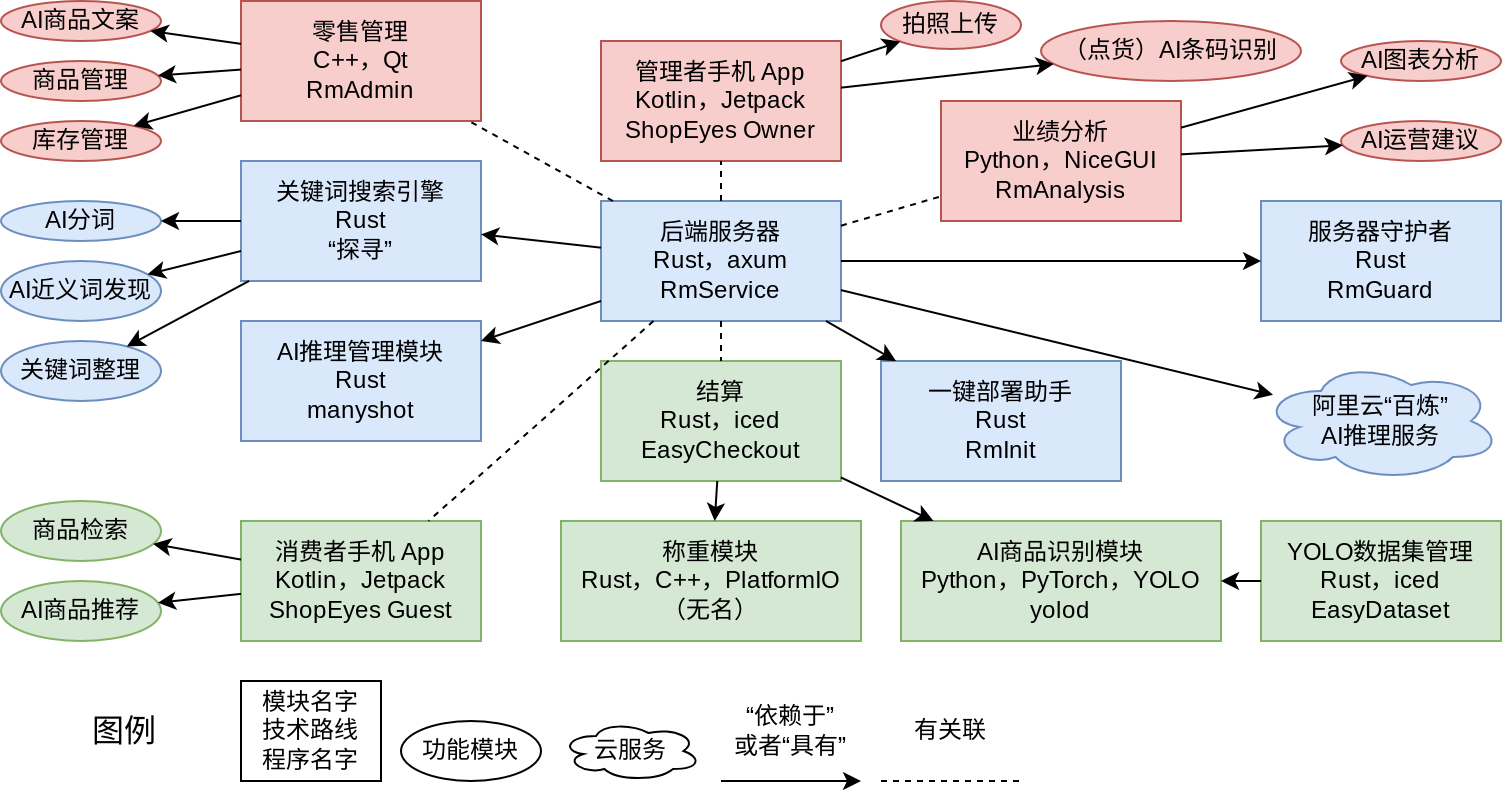
\includegraphics[width=0.8\textwidth]{./imgs/structure2.png}
	\caption{本设计的系统架构图示。其中蓝色部分为服务端,红色部分为商家端、绿色部分为顾客端。图例(不同形状的各自意义)位于图像下侧。}
	\label{fig:structure2}
\end{figure}

本设计的系统架构如图 \ref{fig:structure2} 所示,而从图像中不难看出,该系统整体上呈现出客户端-服务器模式的结构,其中客户端部分分为面向零售行业从业者的商家端和面向最终消费者的顾客端。

\subsection{服务端}

本设计中对服务端功能的期望主要有如下几点:

\begin{enumerate}
    \item 高性能的HTTP API服务器
    \item 商品、库存、订单等运营资料的增删改查
    \item 高性能、效果良好的智能商品搜索
    \item AI大语言模型推理托管
\end{enumerate}

实际部署的情况下,服务器可能需要在短时间内处理来自大量客户端应用程序的服务请求,比如营业高峰期来自许多客人的商品检索、询问AI助手索取导购建议的请求,因此服务器本身的效率必须纳入设计的考虑之中。基于这样的考虑,该设计采用Rust语言进行开发。Rust是比较流行的一门强调内存安全的系统编程语言,利用这门语言,服务器的代码执行效率有充足的优化机会,并且开发的便利性得到了一定保证。为了充分利用大部分部署环境都将会具备的多处理器的对称并行处理(SMP)执行环境,服务器内主要采用由tokio第三方库驱动的异步开发的技术手段。为了实现服务器与客户端的有效、高效、泛用性强的信息双向传输,采用通过(商铺内部)局域网的HTTP。为了与总体的技术选择相统一,采用依托并行计算技术开发的axum HTTP服务器框架。

服务器需要能实际储存并处理在零售运营过程中需要的各种数据。为了满足这个期望,该设计中采用基于SQLite关系数据库引擎的rqlite分布式关系数据库管理软件作为原始数据存储、查询和管理的手段。为了提供统一可靠的开发接口,rqlite服务器将只面向服务器软件开放,而客户端任何对实际业务数据的访问都必须通过服务器对其结构化、统一化的封装。

为了实现在众多商品中快速找到顾客所需,服务器需要具备通过(顾客提供的)一段可能和商品本身文字内容不尽相同的搜索语句对商品进行匹配的功能。市面上常见的如Apache Lucene、Elasticsearch等各种相关产品与该设计的相关理念并不匹配:因为较为复杂而不适合在该设计所期望的低成本设备上部署;对中文没有比较针对性的优化,并且搜索对象仅限于搜索目标中出现过的字词。为了解决这个问题,该设计中包含一个由多种人工智能技术驱动的,高效、高匹配率、简明易用的中文特化搜索引擎“探寻”。

鉴于该项目中多处利用到了大语言模型,若是服务器可以向各个客户端软件提供统一的推理接口,将不同模型、不同服务商的区别消除,将有利于项目的整体可用性、可维护性。因此,服务器提供一个专门开发的的推理模块,具备单次推理(“oneshot”)、多次尝试(“manyshot”)和有状态多轮对话管理等功能。

\subsection{商家端}

本设计中对商家端功能的期望主要有如下几点:

\begin{enumerate}
    \item 高性能、便于使用的用户界面
    \item 功能丰富、易于操作的商品、库存管理界面
    \item 完整的销售数据查询界面
    \item 业绩图表生成、展示界面
    \item 业绩图表AI智能分析、运营建议
    \item AI条码识别点货
    \item AI商品文案自动生成、批量生成
    \item 商品识别数据集创建和修改
    \item 从手机上传用于商品的图片
\end{enumerate}

为了在普通的计算机上高效管理营业资料,商家端需要一套对系统要求较小的、对键盘鼠标操作较为友好的,对屏幕尺寸需求灵活的用户界面。基于这样的缘由,该设计的商家桌面端应用程序采用Kotlin作为业务逻辑开发语言以最大化开发效率,进而采用受到工业界广泛采用的Qt Widgets应用程序开发框架在Java、Kotlin语言上的实现Qt Jambi。

在实际操作的情况下,经营者不可避免地将需要对各类数据进行条件细致的筛选。为了满足这样的需要,商家桌面端应用程序为多种不同零售资料的查询准备了既功能丰富,又简单易懂的图形化高级搜索条件拟写工具。

将销售数据按表格列出是简单易行的,但这样的数据展示方式往往无法满足营业者的营业数据分析的需要,图表可以更好地呈现数据之中潜在的结构性和规律性。为了实现这样的功能,本设计采用业界惯用的Python语言作为数据分析的主要语言,利用HTTP API与基于Rust的服务器进行通讯,并采用pandas、numpy等数据科学库展开数据整理工作,利用matplotlib库进行图形的绘制。为了简化开发过程,图表部分的用户界面同样采用Python编写,同时选择NiceGUI用户界面框架实现与上述第三方库更高的整合度。

为了减轻零售从业者观察图形规律的压力,该设计利用来自阿里云“百炼”AI推理服务的多个AI模型,针对不同类型、复杂程度的营业数据图表进行“先观察后思考”的“接力式”智能分析报告编写或者“边观察边思考”的快速图形规律总结,向从业者提供详尽准确的数据分析。

业务资料中的商品图片较为特殊,在手机设备上处理可能相比在桌面型计算机上更加便捷。因此,该项目采用Jetpack Compose安卓应用程序开发框架实现面向商家的管理用应用程序。利用该应用程序营业者可以较为简单地将手机中的照片或现场拍摄的照片上传到服务器中。

实体零售行业常常无法避免对仓库中、货架上产品进行审计(统计),以此确认实际产品数量与系统中库存数量对应关系的需要,而手工记录并比照的方法费时费力并且容易出现错误。因此,该设计的移动商家端应用程序采用谷歌MLKit的AI条码识别功能开发了利用手机自带摄像头的AI条码识别并记录、上传的功能。

为了简化用于智能结算房屋中的商品识别模型的训练工作,该项目具备利用Rust和iced用户界面框架开发的数据集创建和修改功能。数据集准备的过程分为“类别规划”“图片采集”和“图片管理”三个连贯的部分。从业者能够先根据实际的需要在应用程序中输入需要的商品种类,再利用智能商品识别对应的摄像设备进行数据集中图片的采集,最后在采集的图片中筛选出质量较高者。

\subsection{顾客端}

本设计中对顾客端功能的期望主要有如下几点:

\begin{enumerate}
    \item 美观大方、便于使用的用户界面
    \item 推荐商品浏览
    \item 商品检索和详情浏览
    \item AI导购多轮对话商品推荐
    \item 基本商品结算
    \item AI商品识别-计重结算
\end{enumerate}

为了最大程度提高消费者获取商品信息的便利程度,增强新零售购物体验,该项目采用Jetpack Compose开发面向消费者的用于浏览商品情况的应用程序。应用程序分为“推荐”“搜索”和“询问AI”三个板块,分别通过不同的用户界面、不同的对服务器API的请求方式来实现相应的功能。其中推荐功能展示由从业人员在商家端预先设置的一系列推荐商品,而搜索功能顾名思义。

另一个功能是“询问AI”。在该功能界面下,用户可以通过屏幕底部的搜索框输入需要向AI询问的导购相关问题,用户输入的问题将会经由服务器中转发送到后端预先指定的推理服务和选择的大模型。在获取输出之后,顾客端应用程序会利用AI的答复再次利用AI进行关键词的提取,进而利用归纳得出的关键词进行对商品的检索,进而实现对用户推荐相关的商品的功能。

为了同时满足店员辅助结算和消费者自主结算的需要,该项目需要提供一个用于结算设备的简洁明了的用户界面。因此,该设计采用Rust语言及iced用户界面开发框架设计开发结算用用户界面。用户可以利用通过人体工学输入设备(HID)方式连接到结算设备的激光条码扫描设备来输入任何按件结算的商品。

某些零售细分领域所提供的商品(如生鲜蔬果、熟食等)是按重量结算的,需要称重才能获取实际价格,并且按实际情况有可能商品表明无法粘贴对应的条形码(比如肉类),需要其他手段辅助才能确定商品的具体类型。为了解决这样的问题,本设计利用YOLO图像分类模型,结合前文提及的商家端数据集管理工具,开发AI智能商品识别算法,用以简化计重商品结算流程。
\newpage
\section{实现细节}

\subsection{零售管理系统总览}
\label{sec:foundation}

\subsection{服务器}

\begin{figure}[htbp]
	\centering
	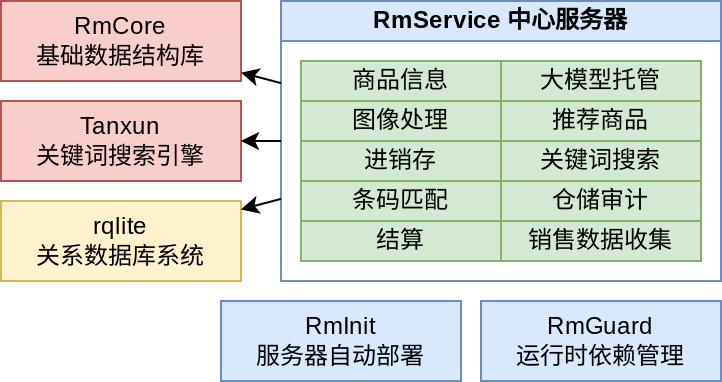
\includegraphics[width=0.8\textwidth]{./imgs/arch-server.png}
	\caption{本设计的服务器整体设计图示:其中蓝色表示相互独立的应用程序,绿色表示服务器的功能,红色表示功能库,黄色表示第三方库或应用程序,箭头表示被指方受到依赖。}
	\label{fig:arch-server}
\end{figure}

\subsubsection{数据结构}
如图 \ref{fig:arch-server} 所示,因为采用了客户端-服务器设计模式,该系统所有业务相关信息统一由RmService模块进行管理。因此,为了在系统中体现充分的可维护性、可拓展性,实际对数据进行存储的关系数据库系统rqlite原则上无法被客户端(各个商家端、顾客端应用程序)所直接访问,而是由RmCore所定义的数据结构进行封装。

\begin{figure}[htbp]
	\centering
	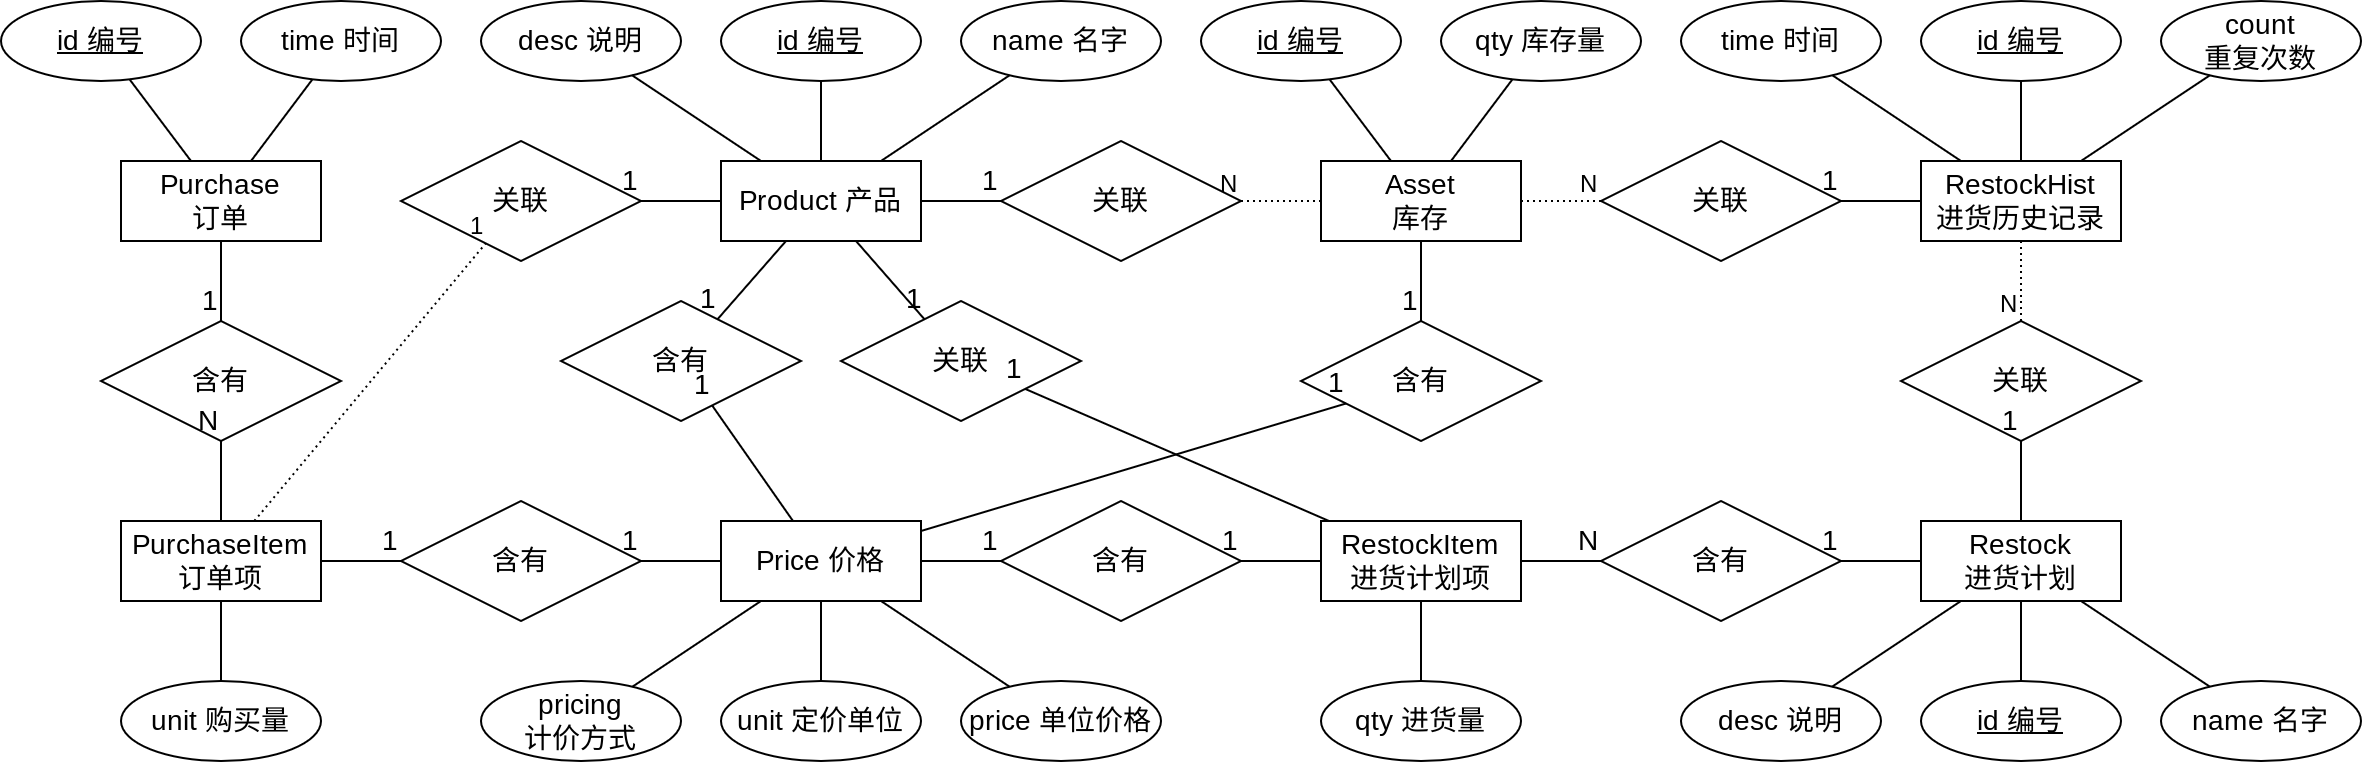
\includegraphics[width=0.8\textwidth]{./imgs/rms-er-rmcore.png}
	\caption{RmCore模块所定义数据结构的实体关系图}
	\label{fig:rms-er-rmcore}
\end{figure}

如图 \ref{fig:rms-er-rmcore} 所示,该模块定义了在零售经营过程中会利用到的各种(需要持久化存储的)数据结构,并且已经以面向对象的、有利于代码复用、序列化和反序列化和有利于在不同开发环境下形成统一接口的方式进行封装。为了便于在数据库中以整数方式存储许多常常为小数的数据,规定任何直接代表金钱数量的值以人民币分为单位,任何直接代表物体质量的值以克为单位。

其中值得注意的一个类型是库存“Asset”。为了便于对库存所对应的进货批次、进货价格等信息进行跟踪,每一个库存项都与一个进货历史记录项目“RestockHist”相关联。因此,同一个产品可以因为多次不同进货并且较老进货批次剩余产品尚未被消化完毕而存在多个库存条目。同样地,只需要统计一个RestockHist所对应的Asset,便可以统计某一个批次进货的消化情况。

另一个较为特殊的类型是价格“Price”。考虑到不同零售商品类型定价策略的区别,该类型的属性计价方式“pricing”为具有“Package”(按件)和“Weight”(按重量)两个可能值的枚举。而属性定价单位“unit”在按件计价时代表属性价格“price”对应的商品件数,反之则是克数。而将属性price和unit分离(而不是表示为单位价格)有助于避免如“十元三件”(一件$\frac{10}{3}$元)此类出现整数或IEEE 754浮点类型数字无法准确表示的数值的情况。

\begin{figure}[htbp]
	\centering
	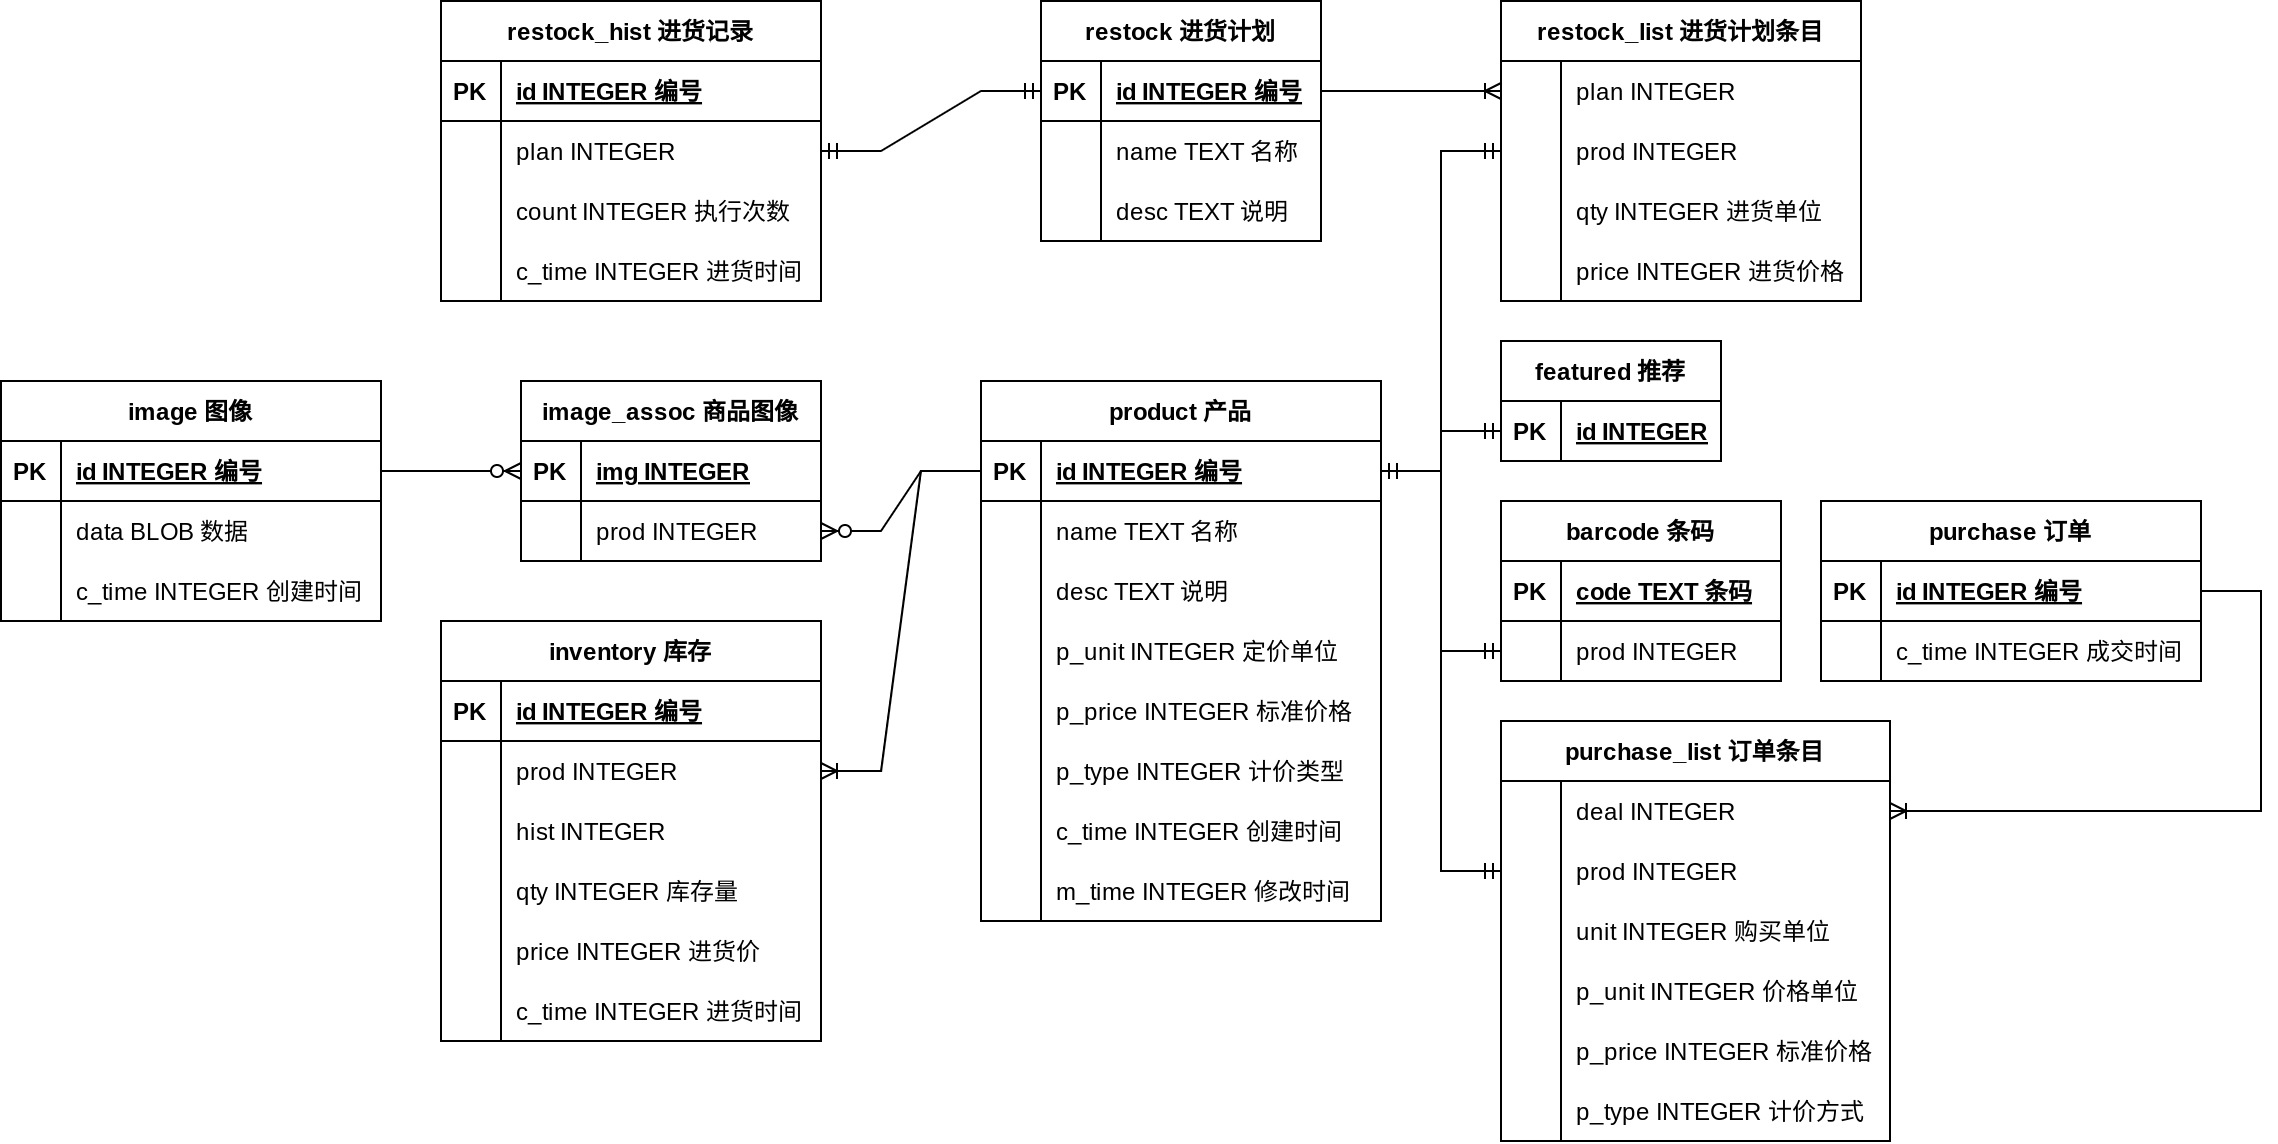
\includegraphics[width=0.8\textwidth]{./imgs/rms-db.png}
	\caption{数据库中存储数据格式的实体关系图}
	\label{fig:rms-db}
\end{figure}

图 \ref{fig:rms-db} 所描绘的是 \ref{fig:rms-er-rmcore} 所示的模型还有少数以其他方式封装的数据的在关系数据库系统中的实际存储方式。除了Price类型没有单独表格,而是被扁平化地存储在了各个表中的区别,数据存储的方式基本与封装成一比一对应关系。少部分表格具有额外的创建、修改时间字段(“\verb|c_time|”和“\verb|m_time|”)留作未来拓展使用。值得注意的是,为了改善大规模访问的效率,商品图像数据并不是存储在外部文件系统,而是和其他资料一同存储在数据库中。

\subsubsection{应用程序接口}
为了实现各个客户端应用程序与服务器的有效信息交换,服务器采用HTTP协议进行信息传递,即服务器实现面向客户端应用程序的HTTP API。由于API覆盖范围较广、数量较大并且功能迥异,故该课题代码开发时大部分API端点设计遵从如下规范:

\begin{itemize}
	\item 期望请求主体(body)部分带有实际数据者,接受POST方法的请求;否则接受GET方法的请求,并且对方法错误的请求响应“Not Found”状态。
	\item 期望请求主体带有多于一个字段者,接受使用JSON格式序列化的数据,否则按实际情况决定主体数据类型。
	\item 较短、较少的请求参数,可以通过HTTP地址参数而不是请求主体传递。
	\item 除纯二进制数据(如图片)外,方法一律使用JSON格式序列化返回值。
	\item 在端点调用遇到责任在客户端(调用参数格式错误等)的问题时,返回“Bad Request”状态并且尽可能在回复主体中包含对问题根源进行描述的字符串。
	\item 同上,但责任在服务器(意外情况)时,返回“Internal Server Error”状态并且在主体中包括导致问题的函数调用返回的相关错误信息。
	\item 客户端请求的资源或任务结果尚未准备完成时,返回“Accepted”状态并在回复主体中标注具体任务现状。
\end{itemize}

为了支持商家端应用程序中对某些数据条目的高级搜索功能,服务器对某些数据类型提供了封装程度较低的请求方式,即允许部分客户端应用程序自行合成并向服务器提供用于数据获取的SQL查询 \verb|SELECT| 调用参数中的 \verb|WHERE| 子句。值得注意的是,该特性因为受到的自动检查、合法性担保较少而具有一定的危险性,不合理的使用可以引发较严重的安全隐患。因此,只有特定商家端的功能将会使用到这个API终点,并且子句的合成也会(在客户端)受到一定的规范和限制。

\subsubsection{自动部署}
不难发现,该设计所实现功能板块领域跨度较大,在原理、技术路线和使用环境要求上不尽相同,甚至在某些情况下相差甚远,所以部署的难度和复杂程度是比较高的。因此,该设计包含一个利用与服务器相似的技术路线开发的自动服务器部署应用程序RmInit。

该程序具备利用系统命令执行和命令输出检测该设计中各个功能模块在该程序所运行的设备上运行所依赖的第三方软件库或执行环境是否正确安装的功能;具备使用系统自带下载工具(如 \verb|wget| )自动从互联网上下载对应该程序所运行的设备的体系结构的rqlite应用程序合集,并且在部署的系统上运行数据库初始化脚本的功能;能够按照预先准备的应用程序项目列表逐个运行对应的编译任务并复制编译输出的二进制程序,支持使用 \verb|uv| 托管的Python项目、使用Gradle项目管理工具的Java-Kotlin项目、基于CMake项目管理工具的C++项目和使用Cargo命令管理的Rust可执行程序项目目标。

为了适应在多设备分布式系统中正确分配各设备功能特性、规避在特定平台无法完成编译任务的应用程序,RmInit采用了 \verb|clap| 命令行参数分析器,支持利用命令行参数控制大部分功能的包含与否、部分配置文件的覆盖与否。

此外,该应用程序还实现了可选的配置文件升级功能。配置文件升级是一个递归的过程,每一次调用都由新配置和旧配置(或者它们的一部分)参与。若新旧配置均为基本值类型且类型一致,则旧配置受到保留。若新旧配置类型、结构不一致,则使用新配置取代之。若新旧配置为键值表,则利用旧表内容覆盖新表,每个元素的覆盖递归执行该过程。

\subsubsection{服务依赖管理}
服务器中不同应用程序可能存在一定依赖关系,比如RmService依赖于rqlite关系数据库管理系统,此时合理安排各个应用程序或后台服务的启动顺序对系统整体稳定程度将会有所帮助。因此,服务器工具软件中包含RmGuard服务器运行时依赖管理,支持按网络请求启动或停止相关服务的服务器守护程序。该应用程序内置服务器中不同模块二进制程序之间的依赖关系,并且启动时将会读取对应的配置文件。不论使用任何方式(自启动或按需启动)来唤起任何模块,都会触发对应程序所依赖的模块(若尚未启动)的启动过程。

\subsubsection{图像存储}
为了顺利在较为受到限制的存储空间内存放潜在的海量商品图像,并且改善各应用程序获取商品图片的速度、降低网络带宽压力,服务器具备自动对图像进行缩放和压缩的功能。服务器所接受的图片(已编码的数据)首先会被解码,然后将被在保持图片原本宽高比的情况下,将图片较长一边的长度限制在300以内,并按需调整另一边,并利用较为快速的双线性插值办法进行重采样。程序将逐个尝试100、95、90\ldots60、55的JPEG压缩率对图片进行编码,直到使用了最大压缩率或图像大小小于配置文件制定阈值为止。

\subsection{管理界面}

\begin{figure}[htbp]
	\centering
	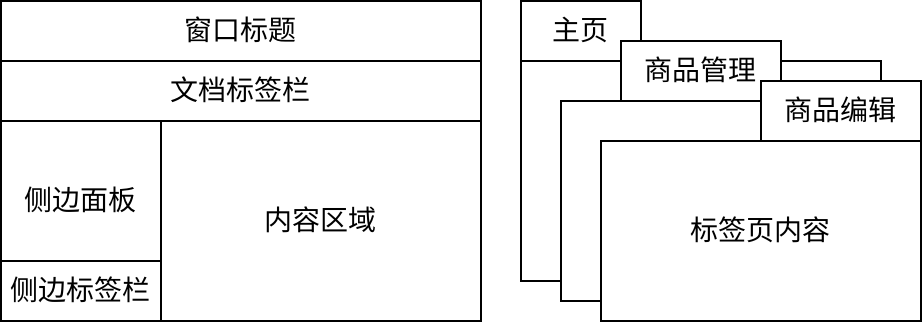
\includegraphics[width=0.8\textwidth]{./imgs/rma-design-layout.png}
	\caption{左侧:桌面商家端的用户界面布局;右侧:多个文档标签的实例}
	\label{fig:rma-design-layout}
\end{figure}

为了充分利用面向桌面型计算机开发的应用程序的操作效率高的特性,管理界面模块采用如图 \ref{fig:rma-design-layout} 所示的按标签页分文档的UI组织方式,其中大部分标签页采用主要内容板块加侧边栏展示额外信息的布局方式,以增强对键盘鼠标操作的友好性。鉴于许多种类的零售业务资料可以被抽象为同一种类型的多个不同实例,并且具有同样的对理解数据内容较为重要的字段(如名称、说明),故决定以表格方式对其进行整理。管理界面具备如下的功能:

\begin{itemize}
	\item 商品管理
	\begin{itemize}
		\item 创建或编辑商品
		\item 检索、查看和管理既有商品
	\end{itemize}
	\item 库存管理
	\begin{itemize}
		\item 管理、预览和执行进货计划
		\item 查看仓储情况
		\item 管理仓储审计批次
	\end{itemize}
	\item 编辑推荐商品
	\item 管理商品图片
\end{itemize}

\begin{figure}[htbp]
	\centering
	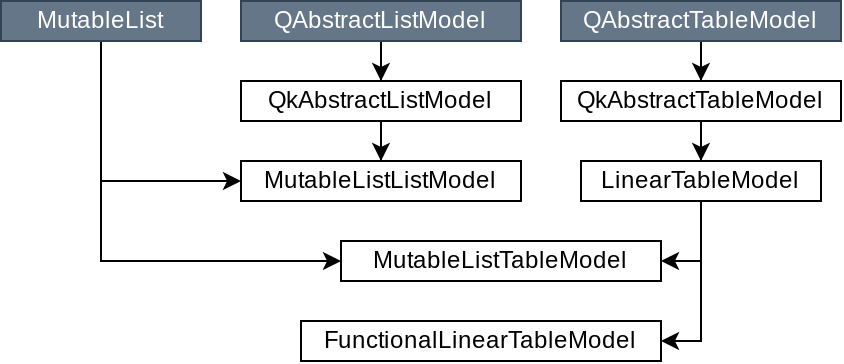
\includegraphics[width=0.8\textwidth]{./imgs/rma-tables.png}
	\caption{用于表格组件的模型类继承关系:灰色框代表第三方库或开发环境带有的类,箭头指向子类或者实现该接口的类。}
	\label{fig:rma-tables}
\end{figure}

不同表格模型(向表格组件提供数据的对象)类之间的继承关系如图 \ref{fig:rma-tables} 所示,其中 \verb|MutableListListModel| 和 \verb|MutableListTableModel| 在表格模型中整合了可变不定长数组的特性,可以将开发模型中的对象数组与对应对象集合在UI上的展示相同步,避免繁重的界面开发任务,以此简化数据映射的开发复杂程度。

此外,管理界面的许多作为既有信息展示方法的表格组件还具备通过键盘快捷键或右键菜单进行搜索结果整理、复制或粘贴的功能,从业者可以通过在不同的搜索结果、功能模块之间粘贴剪贴板中编码的对象引用来实现较为复杂的查询和修改。例如若需要查询某几种商品的库存情况,可以首先在“商品管理”中对所需商品进行检索,再在该界面内复制所需商品,在库存查询界面粘贴,即可查看对应的库存情况;若需要在编辑商品信息的过程添加图片,可以在图片管理界面检索到所需的图片,在将图片(的引用)复制到商品编辑所对应的标签页。

\subsubsection{高级搜索}

\begin{figure}[htbp]
	\centering
	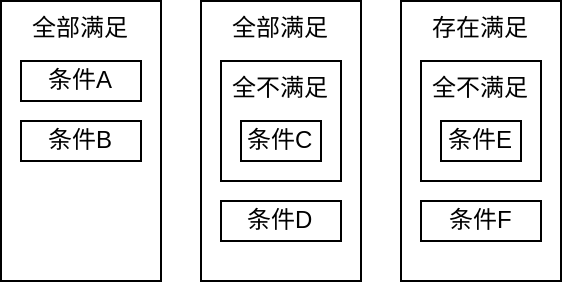
\includegraphics[width=0.8\textwidth]{./imgs/rma-design-adse.png}
	\caption{复合查询条件示例:三个条件分别等价于$ A \land B $,$ \neg C \land D $和$ E \lor F $}
	\label{fig:rma-design-adse}
\end{figure}

零售业务运作的时候,从业者往往需要从数量较为庞大的数据中筛选出所需的一小部分。为了满足这样的需要,管理界面对某些数据类型提供基于布尔代数思想的复合查询条件设计工具。因此从业者并不需要编写布尔代数表达式或SQL \verb|WHERE| 子句就能进行条件复杂查询操作,通过使用鼠标在应用程序提供的用户界面上操作,从业者可以自由组合以下几种类型的条件(\verb|Criterion|):

\begin{itemize}
	\item 字符串字段:前缀为、后缀为、等价于或包含指定字符串
	\item 数值字段:等于、大于、小于指定数值
	\item 日期时间字段:早于、晚于指定日期时间组合
	\item 编号字段:包含于指定正整数集合
	\item 以上条件的集合:其中元素全部符合、任意符合、全不符合、任意不符合
\end{itemize}

输入完成之后,若应用程序没有检测到非法值,将会生成对应的SQL \verb|WHERE| 子句并发送到服务器,服务器将按照对应语句运行SQL查询并返回结果。例如查询名称(\verb|name|)包含“可乐”二字,并且于2025年4月创建(\verb|c_time|)的商品,与以下SQL \verb|WHERE| 子句近似的语句将会被产生:

\begin{verbatim}
	(name like '%可乐%' and c_time > 1743350399 and c_time < 1746028800)
\end{verbatim}

\subsubsection{移动端程序}

\begin{figure}[htbp]
	\centering
	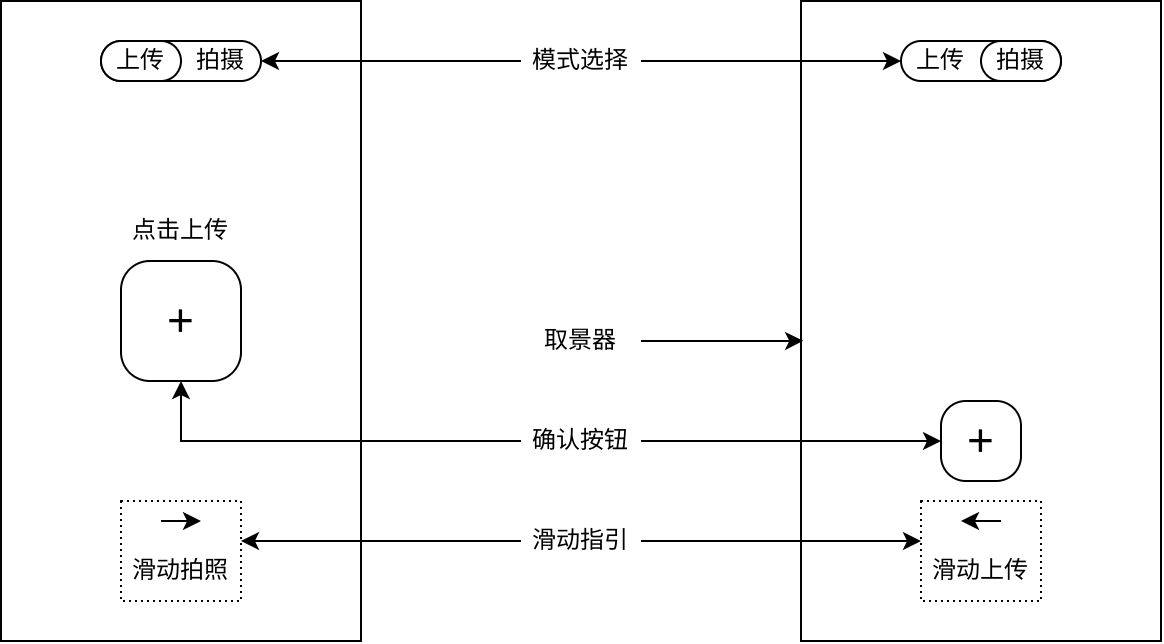
\includegraphics[width=0.8\textwidth]{./imgs/se-picture.png}
	\caption{商家端移动应用程序图像上传部分UI设计}
	\label{fig:se-picture}
\end{figure}

为了进一步降低营业成本,该设计包含一个利用Kotlin语言和Jetpack Compose用户界面库开发的商家端应用程序,用以简化向系统提供图片的流程。从图 \ref{fig:se-picture} 可见,用户可以通过屏幕上侧的标签栏或滑动屏幕空白部分来在上传本地图片和拍摄新照片的界面之间切换。在上传界面上,点击确认按钮可以唤起图片选择界面,用户可以选择一个或多个图片进行上传;在拍摄界面,UI背景部分为取景器画面,在选择完成拍摄角度之后用户只要点击确认按钮即可拍摄照片并即刻上传。

\subsection{结算界面}

该设计具有采用Rust语言和iced实验性用户界面框架构建的用于结算的应用程序。该程序通过与条码识别器、质量传感器和摄像头交互来实现获取商品数据,其后可以在其用户界面上展示待结算的产品。由于具备相应的软硬件支持,该程序可以进行不同计价方式的商品(按件和按质量)的混合结算,一定程度减轻了店员结算的压力和用户自主结算的门槛。

\subsubsection{条码识别器}

为了实现高效识别(计件)商品,结算程序默认通过使用USB HID协议通讯的激光条码识别硬件来读取商品条形码。这种硬件将模拟键盘输入条形码内容,应用程序在商品结算界面将检测是否在较短时间之内从键盘输入符合EAN(European Article Number)-13格式的数据,并在需要时与服务器进行通讯。因为服务器存储条形码的方式是使用字符串而不是数字等其他格式,条形码格式和输入方式方面该设计具有较高的可拓展性,实际部署的情况可以根据不同零售行业细分领域的实际对其进行调整。

\subsubsection{质量传感器}

通过将质量传感器(带有信息传输接口的“电子秤”)整合到结算设备中,设备将具备直接进行计重商品结算的功能,而不需要额外的硬件或设备来进行称重,也不需要额外编写标签并打印。这样,计重商品的结算也可以完全由顾客自助完成,不需要来自店员的帮助。

该设计理论上对质量传感器的规格和信息传输方式没有要求,只要该硬件提供足以断定价格的精度和稳定程度即可使用。本设计默认使用市面上采用率较高的海芯科技HX711电子秤用模数转换器,该芯片成本较为可控,并且在多种平台上具备成熟生态。值得注意的是,HX711的串行通讯功能对相应频率和延迟的要求较为严格。为了解决此问题,本设计包含Arduino UNO 3微控制器开发硬件上采用C++语言和PlatformIO嵌入式开发技术编写的驱动程序,将HX711的专有输出格式转化为了易于处理的文本格式,并通过USB模拟串行接口终端通讯与计算机(和结算程序)相连接和消息传递,以此实现了称重和调零的功能。
\newpage
\section{商家端AI功能}
\label{sec:owner_features}

面向零售行业从业者的AI特性主要围绕着商品设计和图表分析展开。这两个业务板块实际上是以宣传为目的、以市场需要为导向的文本编纂;对营业中的各项数值在不同时间段中的变化趋势、不同周期的重复规律的研究。显然,不管是专业文本编纂还是销售数据挖掘都一定程度上超出了一般零售行业在店从业人员的能力范围。

对于连锁店或其他类型的多店面实体零售企业,门店可以通过系统联网、数据同步的方式将这两项工作转移到企业本体的研发、市场部门,运用专业文学工作者、数据分析人员的专业能力来缓解这样的矛盾,一定程度上也有助于同品牌店面行为的标准化和品牌形象的塑造。然而,这样的做法为每个特定的店面制定相应的经营策略的成本是较高的,并且将会对企业的相关资源造成较大的压力,但若是将每个店面的数据整合处理协同考虑,又会使得各个店面效率的上限下降。并且,这样的运营模式一定程度上忽视了在店管理人员、其他工作人员对店面及其周边市场情况的了解,没有充分利用到不同类型、不同位置工作人员的具体能力素养。

对于个体户

\subsection{商品设计辅助}

\subsubsection{编写文案}

\subsubsection{建议定价}

\subsubsection{提供额外参考}

\subsection{销售数据分析}

\subsubsection{图表生成}

\subsubsection{图表理解}

\subsubsection{营业策略建议}

\subsection{库存审计}
\subsection{顾客端AI功总览}
\label{sec:guest_features}

\begin{figure}[htbp]
	\centering
	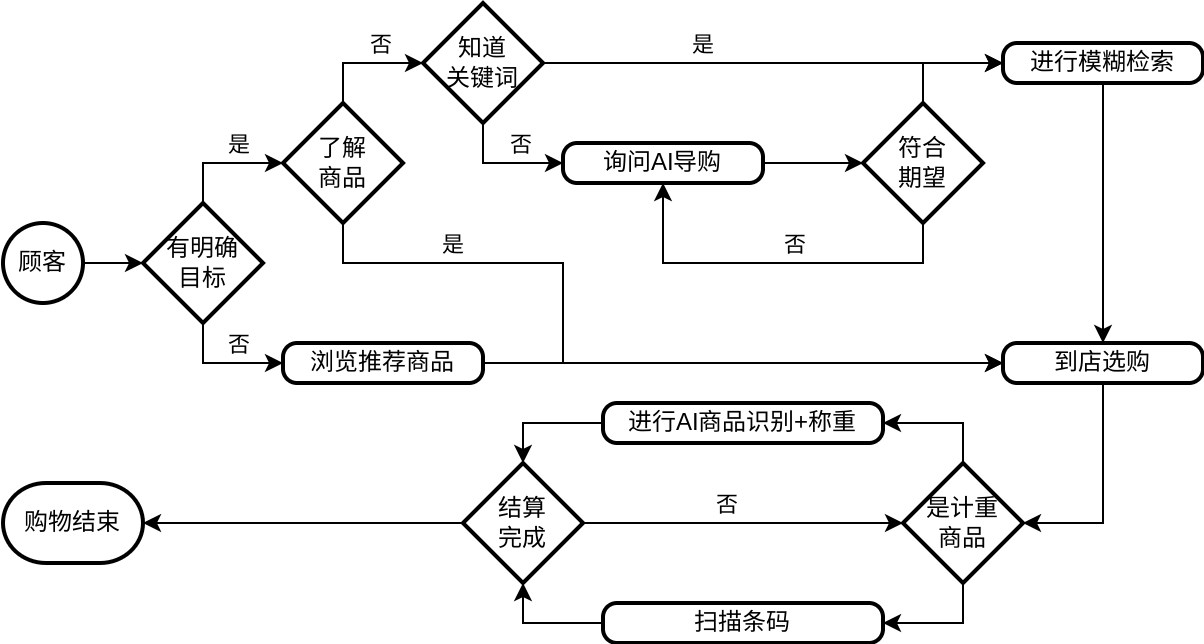
\includegraphics[width=0.8\textwidth]{./imgs/choose-n-buy.png}
	\caption{最终消费者商品选购流程}
	\label{fig:choose-n-buy}
\end{figure}

面向最终消费者的AI功能主要围绕着发现心仪商品和结算所购买商品的场景(如图 \ref{fig:choose-n-buy} 所示)展开。顾客发现商品的方式大致可以分为目的导向的和非目的导向的商品发现方式,其中非目的导向的商品发现方式与商户的宣传手段及其有效性关联较大,很大程度上取决于顾客是否浏览到该商铺对应宣传内容(实体、在线广告、客户群等)和对于宣传内容的实际吸引力。宣传内容的曝光可以由从业人员对社交媒体的参与来实现,而宣传内容可以借助上一部分提及的AI商品文案起草特性来辅助。目的导向的发现方式更为复杂。

目的导向的商品发现方式主要包括用户对商品进行搜索的过程。对于叫法比较单一、名称好记没有歧义的商品,简单分词---匹配的关键词搜索功能是可以满足需要的。然而,时间情况下商品名称匹配的问题可能远复杂于理想的情况。例如笼统和详细说法的区别:“可乐”和“苏打水”都可以叫作“汽水”,但这三个词语之间却无法直接相互匹配,并且若是为此将“汽水”拆为“汽”和“水”,不但仍然无法和“可乐”匹配,还可能会误匹配到与如“水”、“水汽”等词语相关的其他商品。

为了在一定程度上解决该问题,本设计包含模糊搜索引擎项目“探寻”及其对应词典处理脚本。该子项目采用“结巴”分词库\cite{sun_fxsjyjieba_2025,messense_messensejieba-rs_2025}进行分词,并且利用大语言模型对每个词语的近义词进行枚举,最后将各个来源的处理结果整理为高查询效率的格式在为中文优化的自定义搜索算法中进行部署,以此在消耗比较少的计算资源的情况下达到较高的搜索速度和(中文)搜索的准确率,有助于最终消费者更好地进行目的导向的商品发现活动,推动消费体验、营业质量提升。

然而性能更加强大的模糊搜索系统无法解决在许多情况下顾客不知悉需要搜索的关键词(及其近义词)的问题,这种情况下,顾客可能甚至并不清楚自己实际需要的商品。这个问题较为明显的解决思想是使得“商品发现”相关功能具有理解消费者对其需求的描述的语义并将需求内容对应于特定商品信息,或者为此生成对应的搜索语句提供给用户进行检索(或自动运行检索)。

为了解决这种情况带来的问题,该设计的顾客端移动应用程序包含AI导购助手模块。该模块利用经过特定提示词引导的多轮LLM对话及单次LLM调用,分别营造与顾客进行导购交流、导购向用户提出购买建议,如此往复的体验;从导购对用户的回复中提取出适用于检索的关键词语句,以此实现消费者只要合理形容需求,便可检索到对应商品的功能。

AI识别计重商品结算模块是该设计对一般传统实体零售流程的另一个改进。通过利用AI物体识别算法,在零售管理系统中整合物体识别AI模型的训练数据采集、标注等操作对应的用户界面,自动化模型训练和部署的过程;在结算终端中整合AI物体识别前端软件及摄像头、质量传感器等硬件来实现营业者轻松部署AI物体识别模型,最终用户轻松自助结算计重商品,去除计重商品结算过程对店员参与的要求。

\subsection{导购助手}

\begin{figure}[htbp]
	\centering
	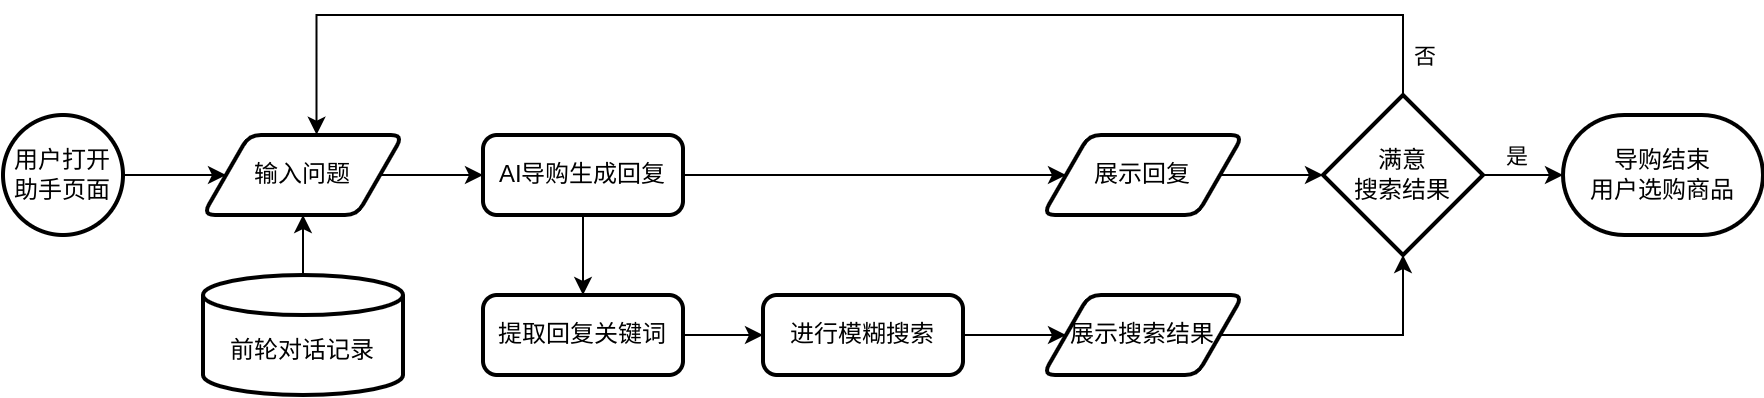
\includegraphics[width=0.8\textwidth]{./imgs/ask-n-choose.png}
	\caption{最终消费者导购操作流程}
	\label{fig:ask-n-choose}
\end{figure}

导购助手工作流程如图 \ref{fig:ask-n-choose} 所示,主要包括以下两个部分:

\begin{itemize}
    \item \textbf{对话式AI导购专家:} 通过与最终消费者的一轮或多轮对话确定消费者的具体需求,并给出相应的购买建议(商品类型、名称等)。
    \item \textbf{搜索关键词猜测算法:} 通过利用大语言模型强大的文字处理能力,使用AI导购的输出产生出对应的搜索关键词。
\end{itemize}

\subsubsection{对话型生成式AI}

AI导购专家实质上就是扮演导购身份,可以与用户进行多轮对话,解决用户困扰的人工智能聊天机器人(chatbot)。为了使得输出较为中性的无(行业相关)微调的一般大语言模型输出符合“导购身份”的回复,而不是一般的建议。该设计主要采用“百炼”的商业大模型 \verb|qwen-turbo| ,开发了以下的系统、对话提示模板:

\begin{itemize}
    \item[] \textbf{系统:}You are a helpful assistant of a retail shop that advise about buying stuffs.\footnote{此处为开发方便(并且遵照“百炼”官方文档中系统提示的风格)使用了英文系统提示,但实际测试中AI发挥了语言中性的能力,正确地使用中文响应了中文编写的输入。若需要中文提示,可以使用:你是零售商店的一个乐于助人的导购,你向客人提出购物建议。}
    \item[] (对每轮对话重复:)
    \begin{itemize}
        \item[] \textbf{用户:}\textit{(提出问题)}
        \item[] \textbf{模型:}\textit{(回复用户提问)}
    \end{itemize}
\end{itemize}

利用这样的对话模板,AI导购助手可以与用户进行(上下文长度范围内的)任意多轮对话,并且每轮对话之间可以产生关联(可以视为大模型聊天机器人的短时记忆特性),从而提高向用户提出正确推荐的概率。同时也因为对话记录参与下一轮对话的特性,应用程序带有由用户手动重置对话的功能,以此避免不同主题、结论的对话记录对新一轮对话大模型推理的干扰。

\subsubsection{搜索关键词提取}

在每一轮对话AI进行回复之后,相应的回复将会作为另一套提示词的一部分输入到模型中,以进行搜索使用的关键词的提取。在该设计对应实现中该特性使用的大模型为“百炼”的商业大模型 \verb|qwen-turbo| 。提示词对话如下:

\begin{itemize}
    \item[] \textbf{用户:}请根据这段话生成一些搜索商品的关键词,并且不要输出任何无关内容:\textit{(该轮对话中大模型的输出)}
\end{itemize}

理论上该过程可以和前文提及进行对话的过程进行合并,但该设计在此次选择将二者分开的设计方式,主要是有两个考量。首先是因为大模型输出难以控制格式的问题,此处避免需要大模型根据JSON等特定的格式输出结果(语义上就是输出两个不同的字符串),以此减轻对大模型推理、服从指引能力造成压力。其次是通过将大模型的输出输入到该任务的大模型(可以为同一个)之中,截断了单次全部输出的模式的标记(token)之间的线性关联,使得关键词的输出不直接受到用户原始输入(和前轮对话)的影响,从而一定程度上提高可预测性和防止模型受到用户特定语义不明确的输入而产生意外输出的问题。

\subsubsection{商品搜索}

\begin{figure}[htbp]
	\centering
	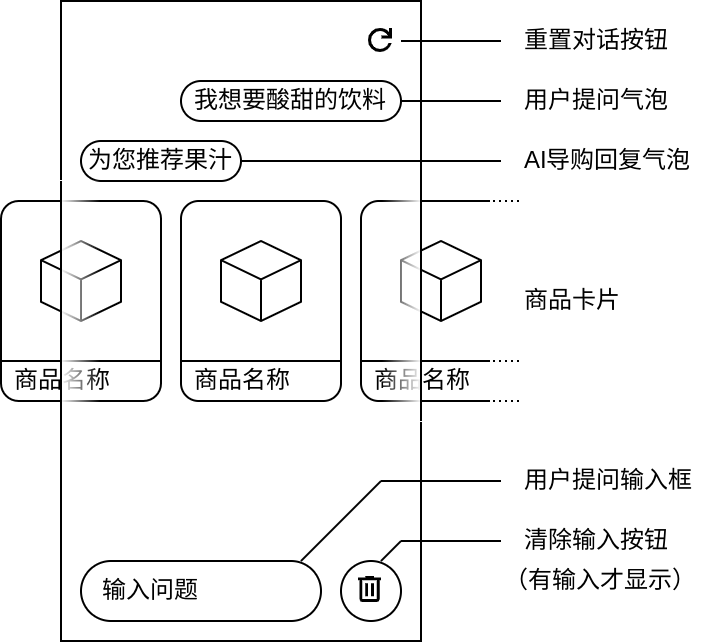
\includegraphics[width=0.8\textwidth, height=0.3\textheight, keepaspectratio]{./imgs/se-assist.png}
	\caption{AI导购用户界面}
	\label{fig:se-assist}
\end{figure}

大模型输出的关键词被用于模糊搜索,搜索结果连同用户的原始输入和AI导购的答复将经过如图 \ref{fig:se-assist} 所示的用户界面展示给用户。值得注意的是,前文提及的使得大模型提取AI导购回答中搜索关键词的输入之中并无对输出(搜索关键词)格式的规定。这是因为将在后文提及的模糊搜索算法是为词组而不是句子优化的,对实际上搜索语句的格式并无要求,仅仅只需要语句中包含期望的关键词。即便大模型忽视了引导(“关键词”)而输出了相关的连贯句子,搜索步骤也可以正常进行。

\subsection{称重商品识别}

在许多类型的零售细分领域中,不可避免地将会遇到按重量计算,而本身并无包装(俗称“散装”)的产品,这些商品包括但不限于在生鲜蔬果、米面粮油和零食糖果等多种类别中的产品。实际上在社会上的许多商场和超市中,消费者在选购这些“散装”商品的时候,由自己完成的步骤只能持续至商品的挑拣和包装。最为重要的称重环节必须由店员帮助完成,并且因为明显地许多这些商品本身无法贴上条码或其他标签,店员需要在容器上粘贴同时记录了商品类型和质量的“静态标签”或与结算系统联网同步的“动态标签”。这种方式既有重复度较高、专业性较低的人工辅助参与,又需要非标准(EAN-13)的商品信息传递记录手段。

为了缓解这个问题,本设计的结算系统包含利用摄像头和AI图像识别技术的智能计重商品结算功能,还配套用于收集、标记训练用数据的应用程序以简化识别模型的创建过程。借此称重设备的功能可以被整合到结算设备之中,使得用户可以轻松自主结算按质量计算价格的商品。

\subsubsection{数据准备}

\begin{figure}[htbp]
	\centering
	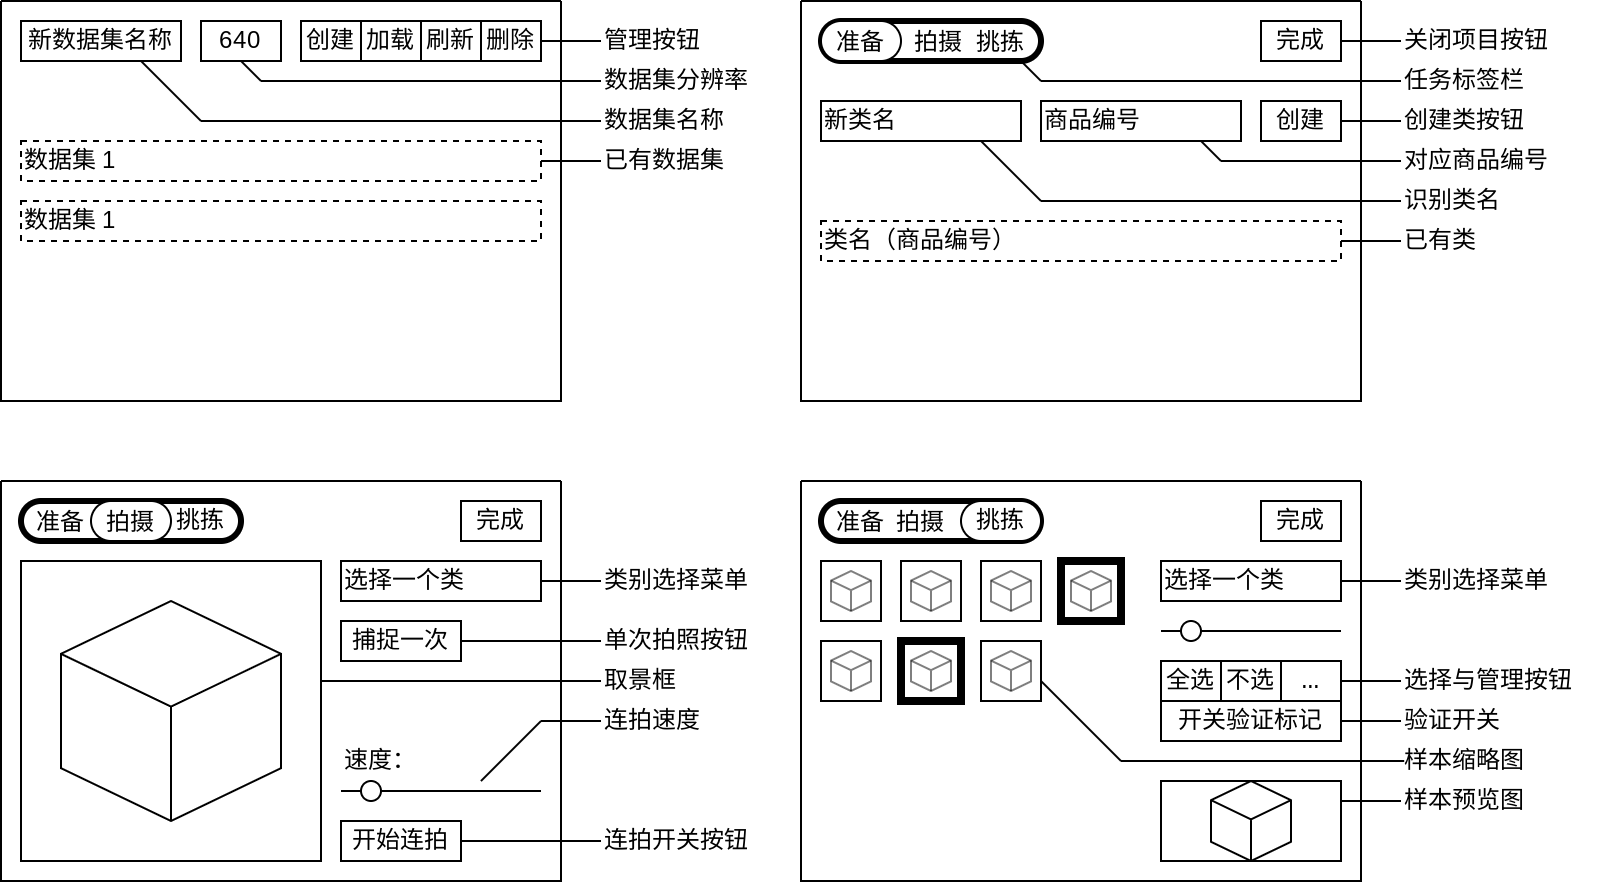
\includegraphics[width=0.8\textwidth]{./imgs/easydataset.png}
	\caption{“EasyDataset”数据集管理应用程序用户界面}
	\label{fig:easydataset}
\end{figure}

如图 \ref{fig:easydataset} 所示,从业者可以在“EasyDataset”应用程序内管理多个不同数据集。在应用程序内打开数据集之后,用户分别可以在“预备”、“拍摄”和“挑拣”三个标签页之间选择需要执行的操作。这三个操作一般情况下为递进顺序。

通过“预备”功能从业者可以准备需要AI识别模型检测到的商品类别列表,其中每个类别具有(隐藏的)类别编号、自身的名称和对应的商品编号。名称将被用于其余两个步骤中选择类别的参考,而商品编号将被用于模型实际部署的场景下结算系统将识别到的类别与具体商品联系起来的过程。此外,点击已经创建完毕的类别可以对其名称或者对应的商品编号进行修改。

使用“拍摄”功能可以为选定的类别拍摄图片。用户首先需要选择对应照片将保存到的类别,然后可以通过点击按钮来完成单张照片的拍摄。为了便于从业者在短时间之内拍摄大量不同角度的照片以提高识别模型的判别性能,该应用程序具有连拍功能。用户可以通过可拖动的调节组件调整连拍速度,其后通过点击按钮可以开始连拍。连拍的过程中用户可以不断调整商品的展示角度、摆放方式,而不需要关注用户界面方面的操作,再次点击按钮可以停止连拍。

针对选中类别,“挑拣”页面将展示已经拍摄的照片。在这个页面,从业者可以批量审阅拍摄完成的样本并从中去除图像素质不符合期望者,点击多个图片可以进行多选批量操作。此外,用户可以通过选中图片之后点击验证开关选择将一部分图片标记为模型效果验证(validation)用的图片,有助于在训练之后检测模型的泛化能力和预计效果。

\subsubsection{图像处理}

该应用程序并不直接保存拍摄的照片。为了考虑到训练和部署环境中可能的区别及数据集在不同版本的商品识别后端(或未来的新版本AI商品识别服务)之间的互换性(interoperability)和兼容性,数据集其中的商品图片统一裁切为以数据集定义时指定的边长的正方形。图片先被以二次线性(或其他更好的)插值算法重采样到短边与指定边长一致的相同长宽比新分辨率,再裁切其中央位置的最大正方形作为最终结果。这样,画面的内容被最大程度保留的同时对模型输入格式的要求较为宽松,并且通过(可选地)重采样到较低分辨率,训练的时间成本可以得到有效的控制,进一步降低使用门槛和维护成本。

\subsubsection{AI图像分类}

\begin{figure}[htbp]
	\centering
	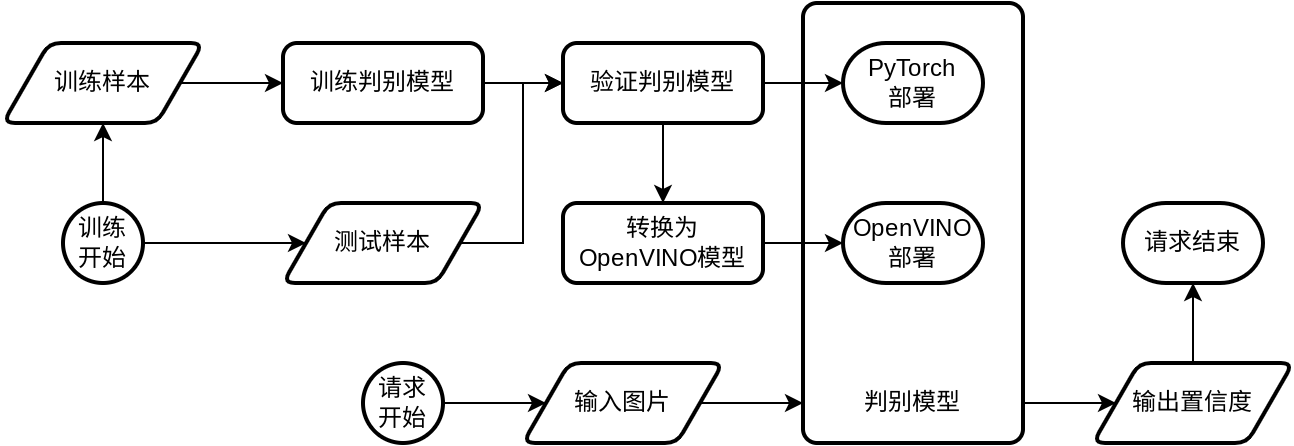
\includegraphics[width=0.8\textwidth]{./imgs/yolod.png}
	\caption{“yolod”图像分类训练-推理服务}
	\label{fig:yolod}
\end{figure}

该设计中提供AI图像分类、分类模型训练的服务“yolod”采用由ultralytics开发的YOLO11(版本 \verb|yolo11n-cls| )图像分类模型\cite{yolo11_ultralytics}作为模型架构,利用在CPU或(可选地)多种不同类型GPU上均可加速运行的PyTorch深度学习框架(版本2.6)和 \verb|ultralytics| 一体式YOLO开发辅助库进行训练和推理任务,利用FastAPI封装推理过程为HTTP API,结算终端应用程序只需要将编码过后的图片发送到yolod,服务器便会自动完成后续处理、推理工作并发回判别结果。

然而,直接使用主要为研究、开发场景优化的原生PyTorch模型进行推理任务效率是不够理想的,常常无法达到商品识别实时性的需要。为了解决这个问题,yolod包含透过\verb|ultralytics|展开的利用英特尔OpenVINO模型优化部署技术执行的推理后端,可以极大地提升推理的效率\footnote{前期实验中OpenVINO上部署的模型相比PyTorch在同样利用英特尔Arc A770 16GB加速硬件推理的情况下展现出了约11倍左右的性能提升。作者推测其中一部分提升幅度是PyTorch的SYCL(oneAPI Level Zero)后端在测试版本上缺乏优化引发的。},最大程度利用CPU或服务器所配置的兼容的加速硬件。值得一提的是,本设计鉴于特定的实验环境作出了使用OpenVINO的决定,但理论上任何有助于模型运行速度提升的部署方式(如ONNX、CoreML等)均可按情况进一步开发,投入使用。

\subsection{模糊搜索}

本设计所包含模糊搜索引擎“探寻”是一个以分词技术为基础,以大语言模型生成近义词作为词典拓展手段开发的、为中文优化的文本关键词模式匹配子系统。该子系统包括用于商品数据处理、AI近义词搜寻、词典构建的脚本和部署在第 \ref{sec:foundation} 部分的搜索算法四个部分。

\subsubsection{商品词典}

商品的搜索实质上是检测商品的标题或说明之中是否含有搜索语句相关模式(词语),同时匹配程度(模式命中次数)较高者更可能符合搜索语句对应语义。在这种情况下,任意一次命中于原文中的位置语义上并无作用,故输出匹配位置的字符串搜索算法并不适合该用途。同时,这也意味着可以快速检测模式是否存在而不包含模式位置相关信息的词典(dictionary)是最适合该用途的数据结构。为了更好传达算法的思想,现列出并解释下文将要直接使用的一些操作和类型:

\begin{itemize}
	\item $F_p$ \textbf{过滤(操作):}该操作接受一个字符串,并返回该字符串移除除了Unicode规范\cite{unicode16.0}所定义的拉丁文字(Latin)、汉字(Han)、假名(Hiragana、Katakana)和谚文(Hangul)以外的文字的版本。
	\item $F_e$ \textbf{扁平化(操作):}该操作接受一个由同元素类型可空集合组成的可空集合,并返回一个由所有原集合中子集合所包含的元素组成的新集合。
	\item $F_c$ \textbf{分词(操作):}该操作接受一个字符串,返回字符串的词语集合。
	\item \textbf{词典(类型):}以字符串(词语或标记)为键,以\textit{以编号数值为键,以频率数值为值的映射}为值的映射类型。
\end{itemize}

以下为根据标记(token)集合生成本模块对应词典数据的算法:

\vspace{1em}
\begin{algorithmic}
	\STATE \textbf{输入:}字符串的集合的序列 $x$
	\STATE \textbf{输出:}词典 $y$
	\STATE $y \gets \emptyset$
	\FOR {\textbf{each} $s$ \textbf{in} $x$ \textbf{of index} $i$}
		\FOR {\textbf{each} $c$ \textbf{in} $s$}
			\IF {$\nexists y(c)$}
				\STATE $y(c) \gets \emptyset$
			\ENDIF
			\IF {$\nexists y(c)(i)$}
				\STATE $y(c)(i) \gets 0$
			\ENDIF
			\STATE $y(c)(i) = y(c)(i) + 1$
		\ENDFOR
	\ENDFOR
\end{algorithmic}
\vspace{1em}

可见该算法遍历了每个条目(商品)对应的字符串(关键词),并对每个关键词在不同商品中的出现进行计数,以此来统计每个关键词与不同商品的关联程度。值得注意的是,该算法对每个商品的输入要求是关键词的集合,根据每个商品的名称和说明生成词语序列的算法如下:

\vspace{1em}
\begin{algorithmic}
	\STATE \textbf{输入:}商品名称和说明的二元组的序列 $x$
	\STATE \textbf{输出:}字符串的集合的序列 $y$
	\STATE $y \gets \emptyset$
	\FOR {\textbf{each} $(a, b)$ \textbf{in} $x$ \textbf{of index} $i$}
		\STATE $s \gets F_e(F_c(a) \cup F_c(b))$
		\STATE $s \gets \{F_p(x) \mid x \in s\}$
		\STATE $s \gets \{x \in s \mid x \neq \emptyset\}$
		\STATE $y \gets y \cup \{s\}$
	\ENDFOR
\end{algorithmic}
\vspace{1em}

由此可知该算法对商品的名称和说明都进行了分词操作,并将分词结果整合为一个序列,按输入的(商品)顺序进行分类,便于后续处理。

\subsubsection{AI近义词搜寻}

为了缓解上文提及的搜索算法无法理解搜索语句(及其单独词语)的语义从而无法搜索到意思相关的词语的问题,此处设计利用大语言模型优秀的自然语言处理能力进行前文提及的词典的拓展。考虑到词语数量可能较为庞大,云端处理的成本是较大的,此处使用本地部署的 \verb|qwen2.5-3b| 模型,提示词对话如下:

\begin{itemize}
	\item[] \textbf{用户:}输出这个词语的所有近义词为JSON字符串集合,不要输出无关内容:
	\item[](原词语)
\end{itemize}

通过在所有词语上重复该操作,并指定模型输出格式(schema)为JSON字符串数组,可以获得每个词语对应的近义词集合。此外,通过多次执行在所有词语上的遍历可以增加获得到的近义词集合的大小。值得注意的是,这种方法一定程度上依赖于模型对指令的遵从能力,并且生成的词语可能需要进一步分词、过滤操作才能用于后续处理。

\subsubsection{近义词词典}

现定义类型“近义词词典”为从词汇到其近义词集合的映射。为了便于实现搜索算法,现定义任何一个词语都是其本身的近义词,因此近义词词典的初始化方法是获取词典中的全部词语,并构建一个对全部词语,以该词语作为输入得到只有这个词语一个元素的集合的映射。生成近义词词典算法如下:

\vspace{1em}
\begin{algorithmic}
	\STATE \textbf{输入:}AI模型生成的近义词词典 $x_1$ ;词典 $x_2$
	\STATE \textbf{输出:}近义词词典 $y$
	\STATE $y \gets \emptyset$
	\FOR {\textbf{each key} $k$ \textbf{in} $x_2$}
		\STATE $y(k) \gets \{k\}$
	\ENDFOR
	\STATE $\hat{y} \gets \{x \mid \exists y(x), \lvert x \rvert \geq 4 \}$
	\FOR {\textbf{each key} $k$ \textbf{in} $y$}
		\STATE $\hat{y}_k \gets \{x \in \hat{y} \mid k \supset x \}$
		\STATE $y(k) \gets y(k) \cup F_e(\{y(x) \mid x \in \hat{y}_k\})$
	\ENDFOR
	\FOR {\textbf{each key} $k$ \textbf{in} $y$ \textbf{if} $\lvert k \rvert \geq 4$ \textbf{and} $x_1$}
		\FOR {\textbf{each} $v$ \textbf{in} $y(k)$}
			\IF {$\nexists y(v)$}
				\STATE $y(v) \gets \emptyset$
			\ENDIF
			\STATE $y(v) \gets y(v) \cup \{k\}$
		\ENDFOR
	\ENDFOR
\end{algorithmic}
\vspace{1em}

从算法上可以看到,首先 $y$ 被初始化为词语到其本身的映射,而后对任何字节长度大于4(一般可视为大于两个中文字符)的字符串,任何被其包含的其他词语对应的近义词都会被添加到该词语对应的近义词集合中(以弥补潜在分词不够细致的问题)。而后同样对任何字节长度大于4的词语其本身都将被添加到其每个近义词对应的近义词集合中,同时将会将这些词语添加为AI生成的近义词词典中对应近义词的近义词集合中。

\subsubsection{搜索算法}

在部署到服务器的搜索算法中,顾客发出的搜索语句首先会被分词和过滤,经过这些操作之后剩余的词语将会被用于实际匹配,搜索算法如下:

\vspace{1em}
\begin{algorithmic}
	\STATE \textbf{输入:}近义词词典 $s$ ;词典 $d$ ;搜索词集合 $x$
	\STATE \textbf{输出:}按匹配程度排序的商品编号序列 $y$
	\STATE $f \gets \emptyset$
	\FOR {\textbf{each} $w$ \textbf{in} $x$}
		\IF {$\exists s(w)$}
			\STATE \textbf{continue}
		\ENDIF
		\STATE $a \gets s(w)$
		\FOR {\textbf{each} $\hat{w}$ \textbf{in} $a$}
			\IF {$\exists d(\hat{w})$}
				\STATE \textbf{continue}
			\ENDIF
			\STATE $m \gets d(\hat{w})$
			\FOR {\textbf{each key} $k$ \textbf{in} $m$}
				\IF {$\exists f(k)$}
					\STATE $f(k) \gets 0$
				\ENDIF
				\STATE $f(k) \gets f(k) + m(k)$
			\ENDFOR
		\ENDFOR
	\ENDFOR
	\STATE \textbf{sort} $f$ \textbf{by value} 
	\STATE $y \gets \{x \mid \exists f(x)\}$
\end{algorithmic}
\vspace{1em}

对每个词语,首先从近义词词典查询其对应的近义词列表(由前文可知该列表可能包含该词语本身),若无结果,则说明该词语在所有商品文字的词语(及其近义词)中尚未出现,可以被安全忽略。否则,针对每一个近义词若词典之中有相应的项目其中所有商品编号对应的词频将会被累加到一个映射中,最后根据总词频对其进行排序,输出排序后的商品编号序列。

\subsubsection{时间复杂度}

以上提及的利用部署词典的搜索算法可以被总结为这样的过程:对每个词语在近义词词典中找到与该词语相关的(词典中的)所有词语,而后对产生的每个词语,逐个将其在每个商品(如果有)中的频率加到结果映射的对应值中。总结起来,这个算法于最坏情况下的时间复杂度如下:

\begin{equation}
	T = O(\log n_s + n_p \times \log n_s \times \log n_d)
\end{equation}

其中 $n_s$ 为近义词词典的元素数量,$n_p$ 为商品数量,$n_d$为词典中的元素数量。考虑到多种情况,实际达到最坏情况的可能性是较小的,达到较为良好的情况可能性更大:所谓关键词即是将某一类商品与其余商品区分开来的词语,因此“这个词语每个商品都有”的情况是比较少见的(比如“的”,但一般不将此字作为关键词看待),因此作者估计 $n_p$ 的影响将较小。

% \newpage
\section{实验}
\label{sec:experiment}

\subsection{商家端}

\subsubsection{桌面应用}

\subsubsection{手机应用}

\subsubsection{数据集管理程序}

\subsection{顾客端}

\subsubsection{手机应用}

\subsubsection{结算程序}
\newpage
\section{讨论}
\label{sec:discussion}

\subsection{AI相关的新功能}

本设计为传统的零售管理系统添加了许多AI相关的功能,功能的类别和设计思想、具体实现和试验效果在前文中已经提及,但为更好总结设计、实现和测试的情况,在此从理解AI在该系统中担任的角色的角度方面再次对实现的功能作出概括。

AI模型可以是“万能函数”。本设计所实现的商品信息生成功能,实质上是输入商品图片等收集难度低的数据,输出商品描述和标题等编写(或收集)难度高的数据,以此来降低从业者数字化转型、维护的负担的功能。也就是从易于获取的数据中提取(由人或算法)较难得出的推论。模糊搜索算法中近义词词典的AI生成过程也是同样的道理,利用固定的词典将会面临较大的局限性,而利用互联网搜索效率较低,但利用从互联网信息训练而来的AI模型则较好地达到了效果和效率上的平衡。

利用AI不能(高效)解决全部问题,但合理利用AI模型有助于在传统算法、函数和人工对接难以处理的情况(常常和自然语言、音视频相关)下达到效率、效果的双重改进。这对于历史上对人工的重复性工作依赖极强的传统实体零售行业,未来的突破和转型具有较大的利用价值。

AI也可以是人工的强化。通过利用AI辅助商品的生成,原本可能在文案编写能力较弱的从业者也可以在不需要外界(如专业写手)的帮助下编写出辞藻丰富的宣传文本。通过利用AI完成导购任务,没有配备专门导购人员的较小商店也有机会达到大卖场的营运效果,这具有大幅强化商店“人-货-场”相匹配的程度的潜力。此外,利用AI识别商品还使得去除店员在称重工作上的参与成为了可能。

当前的AI一般还并不足以或并非被设计用于全面地替代人工,但通过人与AI的协同工作,常常受到限制的人的能力能够得到极大的拓展,同时人的思考也可以一定程度上规避、缓解AI时常会出现的错误。如此,零售行业从业者的负担有望被减轻,同时执行运营事务的门槛也可以得到进一步降低。

\subsection{基本系统的优化}

本设计除了为零售管理系统添加许多AI相关的新功能,还在基本的系统上作出了一些有利于提高营业效率、降低运营成本的改进。其中包括在服务器、数据系统的改善和在用户界面上的改善。

服务器上,本设计采用rqlite分布式数据库系统,充分考虑到了对数据冗余性和多服务端场景下数据库同步的需要。的在数据系统上,本设计采用了库存与进货批次相绑定的做法,保证每次进货都可以追踪到对应的进货批次和进货计划,降低检查、分析的难度。

用户界面上,本设计遵从充分利用不同设备类型固有特性、优势的思想,在桌面端用户界面充分利用鼠标左右键操作和键盘快捷键,提高用户界面的效率和可访问性;在移动端用户界面利用滑动和触摸操作,在许多场景下给用户更多的操作方式选择。

\subsection{“零售商品管理系统”}

本设计实现的是“AI驱动的零售商品全流程管理系统”,没有以已有的管理系统方案作为基底的原因包括现有方案开放程度不足、开源方案对零售行业特化不足(一般为宽泛的CRM、ERP系统)等问题。但最为重要的是,从实验可以看到本设计包含的基本系统虽然体量较小,功能不及商业方案完整,但具备自定义方案的最大优势:与项目目标(AI驱动)的高度协调。本设计所对应系统一定程度上做到了与AI的深度整合和绑定,是目前多数方案所没有做到的。

\subsection{改进空间}

该设计得益于自定义的基本零售管理系统,实现了与AI的高度协同。但也因为开发了自定义的基本系统花费较多的精力和资源,许多AI功能尚有进一步优化、发掘的空间,还有许多潜在的AI功能遗憾地没有得到实现。

较为显著的一个问题是AI生成文字的高度不确定性。AI所产生的输出具有一定的随机性,在提示词或提供的商品信息上的细微的变化也可以使得结果变得完全不一致。不同模型的不同推理、上下文理解性能也可以对生成结果产生极大的影响。虽然带有内省功能的模型(如DeepSeek-R1)可以一定程度上缓解这个问题,但这样会带来极其长的推理时间,许多情况下是不可接受的。这将会是AI与零售相结合必须攻克的一个难关。

另一个较为显著的改进点是AI对零售门店整体情况(门店类型、细分领域等)的总体把握程度。使用完全不了解营业情况的AI相当于让对门店一无所知的人参与管理,这样推理结果的质量必然是较低的。但笼统地直接将门店相关信息、统计数字直接拼接到一个字符串交到大模型的简单方法又会使得效率难以提高,严重浪费计算资源。

合理推断,通过利用带有内省、工具调用功能的AI和智能体(Agent),让AI学会根据需要获取业务资料,统计业务信息,这种问题可以得到一定的改善。
\newpage
\section{结论}

本设计项目立足于传统实体零售行业,致力于探究在传统零售行业中应用、融入乃至于整合人工智能技术,利用人工智能的便利增强经营者的营业能力并降低运营门槛,将更便利的、更有亲和力的实体购物体验带给消费者。

在实现一套完整的基本零售管理系统的基础上,本设计创新地加入了AI商品文案编写、AI驱动的模糊搜索、AI导购助手和AI商品识别等功能,提高了从业者的营业效率和增强了顾客的购物体验。将大模型与基本系统深度整合,本设计探索了“AI+零售”的未来可能性,一定程度上较现有方案更具备创新性。

\subsection{AI相关的新功能}

AI模型可以是“万能函数”。本设计所实现的商品信息生成功能,实质上是输入商品图片等收集难度低的数据,输出商品描述和标题等编写(或收集)难度高的数据,以此来降低从业者数字化转型、维护的负担的功能。也就是从易于获取的数据中提取(由人或算法)较难得出的推论。利用AI不能(高效)解决全部问题,但合理利用AI模型有助于在传统算法、函数和人工对接难以处理的情况(常常和自然语言、音视频相关)下达到效率、效果的双重改进。

AI也可以是人工的强化。通过利用AI辅助商品的生成,原本可能在文案编写能力较弱的从业者也可以在不需要外界(如专业写手)的帮助下编写出辞藻丰富的宣传文本。通过利用AI完成导购任务,没有配备专门导购人员的较小商店也有机会达到大卖场的营运效果,这具有大幅强化商店“人-货-场”相匹配的程度的潜力。此外,利用AI识别商品还使得去除店员在称重工作上的参与成为了可能。

当前的AI一般还并不足以或并非被设计用于全面地替代人工,但通过人与AI的协同工作,常常受到限制的人的能力能够得到极大的拓展,同时人的思考也可以一定程度上规避、缓解AI时常会出现的错误。如此,零售行业从业者的负担有望被减轻,同时执行运营事务的门槛也可以得到进一步降低。

\subsection{基本系统的优化}

服务器上,本设计充分考虑到了对数据冗余性和多服务端场景下数据库同步的需要。在数据系统上,本设计采用了库存与进货批次相绑定的做法,保证每次进货都可以追踪到对应的进货批次和进货计划,降低检查、分析的难度。

用户界面上,本设计遵从充分利用不同设备类型固有特性、优势的思想,在桌面端用户界面充分利用鼠标左右键操作和键盘快捷键,提高用户界面的效率和可访问性;在移动端用户界面利用滑动和触摸操作,在许多场景下给用户更多的操作方式选择。

\subsection{改进空间}

该设计得益于自定义的基本零售管理系统,实现了与AI的高度协同。但也因为开发了自定义的基本系统花费较多的精力和资源,许多AI功能尚有进一步优化、发掘的空间,还有许多潜在的AI功能遗憾地没有得到实现。

较为显著的一个问题是AI生成文字的高度不确定性。AI所产生的输出具有一定的随机性,在提示词或提供的商品信息上的细微的变化也可以使得结果变得完全不一致。不同模型的不同推理、上下文理解性能也可以对生成结果产生极大的影响。虽然带有内省功能的模型(如DeepSeek-R1)可以一定程度上缓解这个问题,但这样会带来极其长的推理时间,许多情况下是不可接受的。这将会是AI与零售相结合必须攻克的一个难关。

另一个较为显著的改进点是AI对零售门店整体情况(门店类型、细分领域等)的总体把握程度。使用完全不了解营业情况的AI相当于让对门店一无所知的人参与管理,这样推理结果的质量必然是较低的。但笼统地直接将门店相关信息、统计数字直接拼接到一个字符串交到大模型的简单方法又会使得效率难以提高,严重浪费计算资源。

合理推断,通过利用带有内省、工具调用功能的AI和智能体(Agent),让AI学会根据需要获取业务资料,统计业务信息,这种问题可以得到一定的改善。

\printbibliography[heading=bibintoc]

\section*{致谢}
\addcontentsline{toc}{section}{致谢}

本设计到此便即将结束,我希望对在这个项目进行设计、开发实现、测试和论文编写过程中给予我帮助的所有人表示由衷的感谢。

首先,我必须感谢该设计的指导老师闫红洋副教授。她严谨、敬业、关心学生成长和未来的教授形象为我和许多其他同学树立了榜样,我相信她的专业精神将成为我们未来工作生活的重要参考和努力目标。

同时,我需要感谢在该过程中向我给予支持、提出建议的其他老师、同组同学、同班同学和其他朋友们,没有他们的热心帮助,我的工作生活将困难许多。我还要感谢我的家人在生活上的各种帮助,没有你们,也就没有今天的我。
% \newpage
% \section*{附录}
% \addcontentsline{toc}{section}{附录}

% \subsection*{配置文件合并算法}

% 
\section{结论}

本文以“外语学习与卧榻之地的跨界融合”为研究对象,探讨了在非传统学习环境中语言习得的效率与身心放松的协同效应。通过理论分析与实践案例的结合,本文提出了一种新型的语言学习模式,即在“卧榻之地”中通过沉浸式体验提升语言能力。研究表明,这种学习模式不仅能够有效缓解学习焦虑,还能通过环境与心理的互动增强语言记忆与应用能力。

\subsection{主要研究发现}
\begin{itemize}
    \item 学习效率的提升:卧榻之地通过降低学习者的疲劳程度($F$)和提升记忆效果($M$)、应用能力($A$)及学习满意度($S$),显著提高了外语学习效率($E$)。
    \item 记忆效果的增强:在卧榻之地中,环境增强因子($E_e$)显著减缓了遗忘速率($k$),从而提高了语言记忆的持久性($P$)。
    \item 学习体验的优化:与传统学习环境相比,卧榻之地提供了更高的时间灵活性和多感官协同体验,使学习者在放松状态下更易进入“心流状态”,从而提升了学习效果。
\end{itemize}

\subsection{研究意义}
本文的研究为语言学习领域提供了一种全新的视角与实践路径。通过将外语学习与卧榻之地相结合,不仅拓展了学习环境的理论边界,还为语言学习者提供了一种更加轻松、高效的学习方式。此外,本文提出的理论模型(如外语学习效率公式、卧榻之地学习效果指数等)为后续研究提供了重要的参考依据。

\subsection{未来研究方向}
尽管本文取得了一定的研究成果,但仍有一些问题值得进一步探讨:
\begin{itemize}
    \item 长期效果评估:本文主要关注短期内的学习效果,未来研究可以进一步探讨卧榻之地学习模式对长期语言能力的影响。
    \item 个体差异分析:不同学习者在卧榻之地中的学习效果可能存在差异,未来研究可以结合学习者的人格特质、学习风格等因素进行深入分析。
    \item 技术辅助优化:随着虚拟现实(VR)和增强现实(AR)技术的发展,未来可以探索如何将这些技术与卧榻之地学习模式相结合,进一步提升学习体验。
\end{itemize}

\subsection{总结}
“外语学习与卧榻之地的跨界融合”不仅是一种学习模式的创新,更是对传统教育理念的挑战与突破。通过本研究,我们希望能够为语言学习者提供一种更加人性化、高效的学习方式,同时也为相关领域的理论研究与实践探索提供新的思路。学外语,不仅要用心,还要用“床”——这或许正是未来语言学习的新方向。

% \printbibliography[heading=bibintoc]
% \section*{致谢}
\addcontentsline{toc}{section}{致谢}

在本论文完成之际,我谨向所有在研究与写作过程中给予我帮助和支持的人表示衷心的感谢。

首先,我要特别感谢我的导师\textbf{高育良教授}。高老师不仅在学术上给予我悉心指导,更以其渊博的学识和严谨的治学态度为我树立了榜样。他常教导我:“学外语,不仅要用心,还要用‘床’。”——这句话不仅启发了我对语言学习环境的思考,也让我深刻理解了理论与实践相结合的重要性。高老师的教诲将伴随我一生,成为我学术道路上最宝贵的财富。

其次,我要感谢\textbf{祁同伟厅长}和\textbf{高小琴女士}。祁厅长在百忙之中为我提供了宝贵的实践机会,让我能够在“卧榻之地”中深入探索外语学习的奥秘。高小琴女士则以其独特的外语学习经验,为我提供了许多灵感和建议。他们的支持与帮助,使我的研究得以顺利进行。

此外,我还要感谢我的家人和朋友们。他们在我研究过程中给予了我无尽的鼓励与支持,尤其是在我“学外语”时,他们总是以理解和包容的态度陪伴在我身边。

最后,感谢所有参与本研究的学习者和实践者。正是你们的积极参与和反馈,才使得本研究得以顺利完成。

谨以此文献给所有在语言学习道路上不断探索的人们。愿我们都能在“卧榻之地”中找到属于自己的学习之道。

\begin{flushright}
\textbf{陈清泉} \\
2025年1月 
\end{flushright}

\end{document}